% Seminar 10: VaR, ES and backtesting
% Statistics of Financial Markets -- Bachelor's programme, Bucharest University of Economic Studies
% GENERATED by latex/build_seminar10.py -- edit the generator, not this file.
% Student version by default; the instructor version is the *_solutions.tex wrapper.
\makeatletter\@ifundefined{ifsolutions}{\expandafter\newif\csname ifsolutions\endcsname}{}\makeatother

\newcommand{\coursename}{Statistics of Financial Markets}
% Preambul comun SFM -- Statistica piețelor financiare / Statistics of Financial Markets (Beamer, 16:9)
% Același design ca MFM. Înainte de % Preambul comun SFM -- Statistica piețelor financiare / Statistics of Financial Markets (Beamer, 16:9)
% Același design ca MFM. Înainte de % Preambul comun SFM -- Statistica piețelor financiare / Statistics of Financial Markets (Beamer, 16:9)
% Același design ca MFM. Înainte de \input{../../latex/preamble} se definește
%   \newcommand{\coursename}{Statistics of Financial Markets}      (EN)
%   \newcommand{\coursename}{Statistica piețelor financiare}       (RO)  și  \def\sfmlang{ro}
% Fișierele .tex se află în EN/Courses, EN/Seminars, RO/Cursuri, RO/Seminarii (două niveluri sub rădăcină).
% Deck-urile sînt generate de latex/build_chapterN.py / build_seminarN.py (vezi latex/sfm_build.py).

\documentclass[9pt, aspectratio=169, t]{beamer}
\providecommand{\coursename}{Statistics of Financial Markets}

% Ensure content fits on slides
\setbeamersize{text margin left=8mm, text margin right=8mm}

%=============================================================================
% THEME AND STYLE CONFIGURATION
%=============================================================================
\usetheme{default}
% Using default theme for clean header/footer control

% Color Palette (matching Redispatch PDF)
\definecolor{MainBlue}{RGB}{26, 58, 110}
\definecolor{AccentBlue}{RGB}{26, 58, 110}
\definecolor{IDAred}{RGB}{205, 0, 0}
\definecolor{DarkGray}{RGB}{51, 51, 51}
\definecolor{MediumGray}{RGB}{128, 128, 128}
\definecolor{LightGray}{RGB}{248, 248, 248}
\definecolor{VeryLightGray}{RGB}{235, 235, 235}
\definecolor{KeynoteGray}{RGB}{218, 218, 218}
\definecolor{SectionGray}{RGB}{120, 120, 120}
\definecolor{FooterGray}{RGB}{100, 100, 100}
\definecolor{Crimson}{RGB}{220, 53, 69}
\definecolor{Forest}{RGB}{46, 125, 50}
\definecolor{Amber}{RGB}{181, 133, 63}
\definecolor{Orange}{RGB}{230, 126, 34}
\definecolor{Purple}{RGB}{142, 68, 173}

% Gradient background (exact Keynote 315° gradient: white to RGB 218,218,218)
\setbeamertemplate{background}{%
    \begin{tikzpicture}[remember picture, overlay]
        \shade[shading=axis, shading angle=315,
        top color=white, bottom color=KeynoteGray]
        (current page.south west) rectangle (current page.north east);
    \end{tikzpicture}%
}
% Fallback solid color for compatibility
\setbeamercolor{background canvas}{bg=}

\setbeamercolor{palette primary}{bg=MainBlue, fg=white}
\setbeamercolor{palette secondary}{bg=MainBlue!85, fg=white}
\setbeamercolor{palette tertiary}{bg=MainBlue!70, fg=white}
\setbeamercolor{structure}{fg=MainBlue}
\setbeamercolor{title}{fg=IDAred}
\setbeamercolor{frametitle}{fg=IDAred, bg=}
\setbeamercolor{block title}{bg=MainBlue, fg=white}
\setbeamercolor{block body}{bg=VeryLightGray, fg=DarkGray}
\setbeamercolor{block title alerted}{bg=Crimson, fg=white}
\setbeamercolor{block body alerted}{bg=Crimson!8, fg=DarkGray}
\setbeamercolor{block title example}{bg=Forest, fg=white}
\setbeamercolor{block body example}{bg=Forest!8, fg=DarkGray}
\setbeamercolor{item}{fg=MainBlue}

% Footer colors (override Madrid theme blue)
\setbeamercolor{author in head/foot}{fg=FooterGray, bg=}
\setbeamercolor{title in head/foot}{fg=FooterGray, bg=}
\setbeamercolor{date in head/foot}{fg=FooterGray, bg=}
\setbeamercolor{section in head/foot}{fg=FooterGray, bg=}
\setbeamercolor{subsection in head/foot}{fg=FooterGray, bg=}

% Bullet styles (apply everywhere including blocks)
\setbeamertemplate{itemize item}{\color{MainBlue}$\boxdot$}
\setbeamertemplate{itemize subitem}{\color{MainBlue}$\blacktriangleright$}
\setbeamertemplate{itemize subsubitem}{\color{MainBlue}\tiny$\bullet$}
\setbeamertemplate{itemize/enumerate body begin}{\normalsize}
\setbeamertemplate{itemize/enumerate subbody begin}{\normalsize}

% Item spacing - compact style
\setlength{\leftmargini}{10pt}       % Level 1: minimal indent
\setlength{\leftmarginii}{10pt}      % Level 2: minimal additional indent
% Compact list spacing (zero extra space before/after lists in blocks)
\makeatletter
\def\@listi{\leftmargin\leftmargini \topsep 0pt \parsep 0pt \itemsep 0pt}
\def\@listii{\leftmargin\leftmarginii \topsep 0pt \parsep 0pt \itemsep 0pt}
\makeatother

\setbeamertemplate{navigation symbols}{}

%=============================================================================
% CUSTOM HEADLINE
%=============================================================================
\setbeamertemplate{headline}{%
    \vskip10pt%
    \hbox to \paperwidth{%
        \hskip0.5cm%
        {\small\color{FooterGray}\renewcommand{\hyperlink}[2]{##2}\insertsectionhead}%
        \hfill%
        \textcolor{FooterGray}{\small\insertframenumber}%
        \hskip0.5cm%
    }%
    \vskip4pt%
    {\color{FooterGray}\hrule height 0.4pt}%
}

%=============================================================================
% CUSTOM FOOTER
%=============================================================================
\usepackage{fontawesome5}

\setbeamertemplate{footline}{%
    {\color{FooterGray}\hrule height 0.4pt}%
    \vskip4pt%
    \hbox to \paperwidth{%
        \hskip0.5cm%
        \textcolor{FooterGray}{\small\coursename}%
        \hfill%
        \raisebox{-0.1em}{%
            \begin{tikzpicture}[x=0.08em, y=0.08em, line width=0.4pt]
                \draw[FooterGray] (0,3) -- (1,4) -- (2,3.5) -- (3,5) -- (4,4) -- (5,6) -- (6,5.5) -- (7,4) -- (8,5) -- (9,7) -- (10,6) -- (11,5) -- (12,6.5) -- (13,8) -- (14,7) -- (15,6) -- (16,7.5) -- (17,9) -- (18,8) -- (19,7) -- (20,8.5) -- (21,10) -- (22,9) -- (23,8) -- (24,9.5);
            \end{tikzpicture}%
        }%
        \hskip0.5cm%
    }%
    \vskip6pt%
}

%=============================================================================
% PACKAGES
%=============================================================================
\usepackage[utf8]{inputenc}
\DeclareUnicodeCharacter{03B1}{\ensuremath{\alpha}}
\usepackage[T1]{fontenc}
\usepackage{amsmath, amssymb, amsthm}
\usepackage{mathtools}
\usepackage{bm}
\usepackage{tikz}
\usetikzlibrary{arrows.meta, positioning, shapes, calc, decorations.pathreplacing, shadings}
\usepackage{booktabs}
\usepackage{multirow}
\usepackage{array}
\usepackage{graphicx}
\usepackage{hyperref}
\usepackage{colortbl}
\usepackage{listings}
\lstset{language=Python, basicstyle=\ttfamily\scriptsize, keywordstyle=\color{MainBlue}\bfseries,
  commentstyle=\color{Forest}, stringstyle=\color{Crimson}, breaklines=true,
  frame=none, backgroundcolor=\color{VeryLightGray}, xleftmargin=2mm}
\hypersetup{colorlinks=true, linkcolor=MainBlue, urlcolor=MainBlue}
\graphicspath{{../../logos/}{../../charts/}{../../photos/}}
\usepackage{xcolor}
\hfuzz=2pt  % Suppress tiny overfull warnings (<2pt)
\vfuzz=2pt  % Suppress tiny vertical overfull warnings (<2pt)

%=============================================================================
% QUANTLET COMMANDS
%   \quantlet{<displayed name>}{<url>}       (generic, compatible with the older SFM decks)
%   \sfmquantlet{Ch_05}{SFM_ch5_garch}       -> https://github.com/danpele/SFM/tree/main/Quantlets/Ch_05/SFM_ch5_garch
%   \qlurl{<folder>} is defined per chapter by the generator (Quantlets/Ch_NN/<folder>)
%=============================================================================
\newcommand{\sfmrepo}{https://github.com/danpele/SFM}
\newcommand{\sfmqlbase}{https://github.com/danpele/SFM/tree/main/Quantlets}
\newcommand{\quantlet}[2]{%
    \hfill\href{#2}{%
        \raisebox{-0.15em}{
\includegraphics[height=0.7em]{ql_logo.png}}%
        \textcolor{MainBlue}{\tiny\ #1}%
    }%
}
\newcommand{\sfmquantlet}[2]{\quantlet{\detokenize{#2}}{\sfmqlbase/#1/#2}}

%=============================================================================
% NOTEBOOKS (Google Colab)
%   \colaburl{notebooks/EN/chapter5_seminar_notebook.ipynb} -> the Colab link of a file in the SFM repo
%   \nb: the chapter notebook (each seminar deck redefines it with \renewcommand)
%=============================================================================
\newcommand{\colaburl}[1]{https://colab.research.google.com/github/danpele/SFM/blob/main/#1}
\newcommand{\nb}{https://colab.research.google.com/github/danpele/SFM/tree/main/notebooks/EN}
\newcommand{\nbname}{notebooks/EN}

%=============================================================================
% SLIDE HELPERS (used by the generators; the same as in MFM)
%=============================================================================
% local font size for list bodies (the preamble forces \normalsize)
\newcommand{\itemsize}[1]{\setbeamertemplate{itemize/enumerate body begin}{#1}\setbeamertemplate{itemize/enumerate subbody begin}{#1}}
\newcommand{\intitle}[1]{{\hypersetup{urlcolor=white}#1}}   % white links inside coloured title bars
\newcommand{\imgcap}[1]{{\scriptsize #1}\\[0.5mm]}          % caption under a photo
\newcommand{\imgcredit}[2]{{\tiny\color{FooterGray}\href{#1}{#2}}}   % image credit: source URL, author/licence
\newcommand{\aiprompt}[1]{{\ttfamily\color{MainBlue}#1}}     % a prompt to an AI assistant

%=============================================================================
% SEMINARS: student version by default; the instructor wrapper *_solutions.tex sets \solutionstrue
%=============================================================================
\makeatletter\@ifundefined{ifsolutions}{\expandafter\newif\csname ifsolutions\endcsname}{}\makeatother
\newcommand{\solonly}[1]{\ifsolutions #1\fi}
\newcommand{\propsub}{\ifsolutions\else\framesubtitle{\ifdefined\sfmlang Rezolvarea se discută la seminar\else Solution discussed in class\fi}\fi}

%=============================================================================
% APPENDIX AND CHAPTER LINKS (latex/appendix_links.py writes the calls; it also re-declares these
% macros before \begin{document}, so the decks compile with or without this preamble block)
%=============================================================================
\providecommand{\sfmapplink}[3]{\hypertarget{#2}{}\hyperlink{#1}{\beamergotobutton{#3}}}
\providecommand{\sfmappback}[2]{\begin{tikzpicture}[remember picture,overlay]\node[anchor=south east] at ([xshift=-3mm,yshift=7mm]current page.south east){\hyperlink{#1}{\beamerreturnbutton{#2}}};\end{tikzpicture}}
\providecommand{\sfmchlink}[2]{\href{#1}{#2}}
\providecommand{\sfmchlinkt}[2]{\href{#1}{\usebeamercolor[fg]{frametitle}#2}}

%=============================================================================
% QUANTINAR COMMAND: link către un curs Quantinar (subiecte avansate)
%=============================================================================
\newcommand{\quantinar}[2]{%
    \href{#2}{%
        \raisebox{-0.15em}{
\includegraphics[height=0.8em]{qr_logo.png}}%
        \textcolor{MainBlue}{\scriptsize\ #1}%
    }%
}

%=============================================================================
% CUSTOM TITLE PAGE
%=============================================================================
\defbeamertemplate*{title page}{hybrid}[1][]
{
    \vspace{0.2cm}
    % Logos row - top header (with clickable links)
    \begin{center}
        \href{https://www.ase.ro}{
\includegraphics[height=1.0cm]{ase_logo.png}}\hspace{0.3cm}%
        \href{https://theida.net}{
\includegraphics[height=1.0cm]{ida_logo.png}}\hspace{0.3cm}%
        \href{https://blockchain-research-center.com}{
\includegraphics[height=1.0cm]{brc_logo.png}}\hspace{0.3cm}%
        \href{https://www.ai4efin.ase.ro}{
\includegraphics[height=1.0cm]{ai4efin_logo.png}}\hspace{0.3cm}%
        \href{https://ipe.ro/new}{
\includegraphics[height=1.0cm]{acad_logo.png}}\hspace{0.3cm}%
        \href{https://www.digital-finance-msca.com}{
\includegraphics[height=1.0cm]{msca_logo.png}}%
    \end{center}

    \vspace{0.6cm}

    % Main title with Q logos on sides (with clickable links)
    \begin{center}
        \begin{minipage}{0.1\textwidth}
            \centering
            \href{https://quantlet.com}{
\includegraphics[height=1.1cm]{ql_logo.png}}
        \end{minipage}%
        \begin{minipage}{0.78\textwidth}
            \centering
            {\LARGE\bfseries\usebeamercolor[fg]{title}\inserttitle}

            \vspace{0.3cm}

            {\usebeamerfont{subtitle}\usebeamercolor[fg]{title}\insertsubtitle}
        \end{minipage}%
        \begin{minipage}{0.1\textwidth}
            \centering
            \href{https://quantinar.com}{
\includegraphics[height=1.1cm]{qr_logo.png}}
        \end{minipage}
    \end{center}

    \vspace{0.6cm}

    % Authors (left aligned)
    \hspace{0.5cm}{\usebeamerfont{author}\insertauthor}

    \vspace{0.3cm}

    % Institute/Affiliations (left aligned)
    \hspace{0.5cm}\begin{minipage}[t]{0.9\textwidth}
        \raggedright\small\insertinstitute
    \end{minipage}
}

%=============================================================================
% THEOREM ENVIRONMENTS
%=============================================================================
\theoremstyle{definition}
\setbeamertemplate{theorems}[numbered]
\ifdefined\sfmlang
\newtheorem{defn}{Definiție}
\newtheorem{thm}{Teoremă}
\newtheorem{prop}{Propoziție}
\newtheorem{rmk}{Observație}
\else
\newtheorem{defn}{Definition}
\newtheorem{thm}{Theorem}
\newtheorem{prop}{Proposition}
\newtheorem{rmk}{Remark}
\fi

%=============================================================================
% CENTRED MINIPAGE (no extra vertical space)
%=============================================================================
\newenvironment{cminipage}[1]{%
    \par\noindent\hfill\begin{minipage}{#1}\ignorespaces
}{%
    \end{minipage}\hfill\null\par
}

%=============================================================================
% CUSTOM COMMANDS
%=============================================================================
\newcommand{\E}{\mathbb{E}}
\newcommand{\Var}{\text{Var}}
\newcommand{\Cov}{\text{Cov}}
\newcommand{\Corr}{\text{Corr}}
\newcommand{\R}{\mathbb{R}}
\newcommand{\N}{\mathbb{N}}
\newcommand{\Z}{\mathbb{Z}}
\newcommand{\B}{\mathbf{B}}
\newcommand{\imark}{\textcolor{MainBlue}{\textbullet}}
\newcommand{\RMSE}{\text{RMSE}}
\newcommand{\MAE}{\text{MAE}}
\newcommand{\MAPE}{\text{MAPE}}

 se definește
%   \newcommand{\coursename}{Statistics of Financial Markets}      (EN)
%   \newcommand{\coursename}{Statistica piețelor financiare}       (RO)  și  \def\sfmlang{ro}
% Fișierele .tex se află în EN/Courses, EN/Seminars, RO/Cursuri, RO/Seminarii (două niveluri sub rădăcină).
% Deck-urile sînt generate de latex/build_chapterN.py / build_seminarN.py (vezi latex/sfm_build.py).

\documentclass[9pt, aspectratio=169, t]{beamer}
\providecommand{\coursename}{Statistics of Financial Markets}

% Ensure content fits on slides
\setbeamersize{text margin left=8mm, text margin right=8mm}

%=============================================================================
% THEME AND STYLE CONFIGURATION
%=============================================================================
\usetheme{default}
% Using default theme for clean header/footer control

% Color Palette (matching Redispatch PDF)
\definecolor{MainBlue}{RGB}{26, 58, 110}
\definecolor{AccentBlue}{RGB}{26, 58, 110}
\definecolor{IDAred}{RGB}{205, 0, 0}
\definecolor{DarkGray}{RGB}{51, 51, 51}
\definecolor{MediumGray}{RGB}{128, 128, 128}
\definecolor{LightGray}{RGB}{248, 248, 248}
\definecolor{VeryLightGray}{RGB}{235, 235, 235}
\definecolor{KeynoteGray}{RGB}{218, 218, 218}
\definecolor{SectionGray}{RGB}{120, 120, 120}
\definecolor{FooterGray}{RGB}{100, 100, 100}
\definecolor{Crimson}{RGB}{220, 53, 69}
\definecolor{Forest}{RGB}{46, 125, 50}
\definecolor{Amber}{RGB}{181, 133, 63}
\definecolor{Orange}{RGB}{230, 126, 34}
\definecolor{Purple}{RGB}{142, 68, 173}

% Gradient background (exact Keynote 315° gradient: white to RGB 218,218,218)
\setbeamertemplate{background}{%
    \begin{tikzpicture}[remember picture, overlay]
        \shade[shading=axis, shading angle=315,
        top color=white, bottom color=KeynoteGray]
        (current page.south west) rectangle (current page.north east);
    \end{tikzpicture}%
}
% Fallback solid color for compatibility
\setbeamercolor{background canvas}{bg=}

\setbeamercolor{palette primary}{bg=MainBlue, fg=white}
\setbeamercolor{palette secondary}{bg=MainBlue!85, fg=white}
\setbeamercolor{palette tertiary}{bg=MainBlue!70, fg=white}
\setbeamercolor{structure}{fg=MainBlue}
\setbeamercolor{title}{fg=IDAred}
\setbeamercolor{frametitle}{fg=IDAred, bg=}
\setbeamercolor{block title}{bg=MainBlue, fg=white}
\setbeamercolor{block body}{bg=VeryLightGray, fg=DarkGray}
\setbeamercolor{block title alerted}{bg=Crimson, fg=white}
\setbeamercolor{block body alerted}{bg=Crimson!8, fg=DarkGray}
\setbeamercolor{block title example}{bg=Forest, fg=white}
\setbeamercolor{block body example}{bg=Forest!8, fg=DarkGray}
\setbeamercolor{item}{fg=MainBlue}

% Footer colors (override Madrid theme blue)
\setbeamercolor{author in head/foot}{fg=FooterGray, bg=}
\setbeamercolor{title in head/foot}{fg=FooterGray, bg=}
\setbeamercolor{date in head/foot}{fg=FooterGray, bg=}
\setbeamercolor{section in head/foot}{fg=FooterGray, bg=}
\setbeamercolor{subsection in head/foot}{fg=FooterGray, bg=}

% Bullet styles (apply everywhere including blocks)
\setbeamertemplate{itemize item}{\color{MainBlue}$\boxdot$}
\setbeamertemplate{itemize subitem}{\color{MainBlue}$\blacktriangleright$}
\setbeamertemplate{itemize subsubitem}{\color{MainBlue}\tiny$\bullet$}
\setbeamertemplate{itemize/enumerate body begin}{\normalsize}
\setbeamertemplate{itemize/enumerate subbody begin}{\normalsize}

% Item spacing - compact style
\setlength{\leftmargini}{10pt}       % Level 1: minimal indent
\setlength{\leftmarginii}{10pt}      % Level 2: minimal additional indent
% Compact list spacing (zero extra space before/after lists in blocks)
\makeatletter
\def\@listi{\leftmargin\leftmargini \topsep 0pt \parsep 0pt \itemsep 0pt}
\def\@listii{\leftmargin\leftmarginii \topsep 0pt \parsep 0pt \itemsep 0pt}
\makeatother

\setbeamertemplate{navigation symbols}{}

%=============================================================================
% CUSTOM HEADLINE
%=============================================================================
\setbeamertemplate{headline}{%
    \vskip10pt%
    \hbox to \paperwidth{%
        \hskip0.5cm%
        {\small\color{FooterGray}\renewcommand{\hyperlink}[2]{##2}\insertsectionhead}%
        \hfill%
        \textcolor{FooterGray}{\small\insertframenumber}%
        \hskip0.5cm%
    }%
    \vskip4pt%
    {\color{FooterGray}\hrule height 0.4pt}%
}

%=============================================================================
% CUSTOM FOOTER
%=============================================================================
\usepackage{fontawesome5}

\setbeamertemplate{footline}{%
    {\color{FooterGray}\hrule height 0.4pt}%
    \vskip4pt%
    \hbox to \paperwidth{%
        \hskip0.5cm%
        \textcolor{FooterGray}{\small\coursename}%
        \hfill%
        \raisebox{-0.1em}{%
            \begin{tikzpicture}[x=0.08em, y=0.08em, line width=0.4pt]
                \draw[FooterGray] (0,3) -- (1,4) -- (2,3.5) -- (3,5) -- (4,4) -- (5,6) -- (6,5.5) -- (7,4) -- (8,5) -- (9,7) -- (10,6) -- (11,5) -- (12,6.5) -- (13,8) -- (14,7) -- (15,6) -- (16,7.5) -- (17,9) -- (18,8) -- (19,7) -- (20,8.5) -- (21,10) -- (22,9) -- (23,8) -- (24,9.5);
            \end{tikzpicture}%
        }%
        \hskip0.5cm%
    }%
    \vskip6pt%
}

%=============================================================================
% PACKAGES
%=============================================================================
\usepackage[utf8]{inputenc}
\DeclareUnicodeCharacter{03B1}{\ensuremath{\alpha}}
\usepackage[T1]{fontenc}
\usepackage{amsmath, amssymb, amsthm}
\usepackage{mathtools}
\usepackage{bm}
\usepackage{tikz}
\usetikzlibrary{arrows.meta, positioning, shapes, calc, decorations.pathreplacing, shadings}
\usepackage{booktabs}
\usepackage{multirow}
\usepackage{array}
\usepackage{graphicx}
\usepackage{hyperref}
\usepackage{colortbl}
\usepackage{listings}
\lstset{language=Python, basicstyle=\ttfamily\scriptsize, keywordstyle=\color{MainBlue}\bfseries,
  commentstyle=\color{Forest}, stringstyle=\color{Crimson}, breaklines=true,
  frame=none, backgroundcolor=\color{VeryLightGray}, xleftmargin=2mm}
\hypersetup{colorlinks=true, linkcolor=MainBlue, urlcolor=MainBlue}
\graphicspath{{../../logos/}{../../charts/}{../../photos/}}
\usepackage{xcolor}
\hfuzz=2pt  % Suppress tiny overfull warnings (<2pt)
\vfuzz=2pt  % Suppress tiny vertical overfull warnings (<2pt)

%=============================================================================
% QUANTLET COMMANDS
%   \quantlet{<displayed name>}{<url>}       (generic, compatible with the older SFM decks)
%   \sfmquantlet{Ch_05}{SFM_ch5_garch}       -> https://github.com/danpele/SFM/tree/main/Quantlets/Ch_05/SFM_ch5_garch
%   \qlurl{<folder>} is defined per chapter by the generator (Quantlets/Ch_NN/<folder>)
%=============================================================================
\newcommand{\sfmrepo}{https://github.com/danpele/SFM}
\newcommand{\sfmqlbase}{https://github.com/danpele/SFM/tree/main/Quantlets}
\newcommand{\quantlet}[2]{%
    \hfill\href{#2}{%
        \raisebox{-0.15em}{
\includegraphics[height=0.7em]{ql_logo.png}}%
        \textcolor{MainBlue}{\tiny\ #1}%
    }%
}
\newcommand{\sfmquantlet}[2]{\quantlet{\detokenize{#2}}{\sfmqlbase/#1/#2}}

%=============================================================================
% NOTEBOOKS (Google Colab)
%   \colaburl{notebooks/EN/chapter5_seminar_notebook.ipynb} -> the Colab link of a file in the SFM repo
%   \nb: the chapter notebook (each seminar deck redefines it with \renewcommand)
%=============================================================================
\newcommand{\colaburl}[1]{https://colab.research.google.com/github/danpele/SFM/blob/main/#1}
\newcommand{\nb}{https://colab.research.google.com/github/danpele/SFM/tree/main/notebooks/EN}
\newcommand{\nbname}{notebooks/EN}

%=============================================================================
% SLIDE HELPERS (used by the generators; the same as in MFM)
%=============================================================================
% local font size for list bodies (the preamble forces \normalsize)
\newcommand{\itemsize}[1]{\setbeamertemplate{itemize/enumerate body begin}{#1}\setbeamertemplate{itemize/enumerate subbody begin}{#1}}
\newcommand{\intitle}[1]{{\hypersetup{urlcolor=white}#1}}   % white links inside coloured title bars
\newcommand{\imgcap}[1]{{\scriptsize #1}\\[0.5mm]}          % caption under a photo
\newcommand{\imgcredit}[2]{{\tiny\color{FooterGray}\href{#1}{#2}}}   % image credit: source URL, author/licence
\newcommand{\aiprompt}[1]{{\ttfamily\color{MainBlue}#1}}     % a prompt to an AI assistant

%=============================================================================
% SEMINARS: student version by default; the instructor wrapper *_solutions.tex sets \solutionstrue
%=============================================================================
\makeatletter\@ifundefined{ifsolutions}{\expandafter\newif\csname ifsolutions\endcsname}{}\makeatother
\newcommand{\solonly}[1]{\ifsolutions #1\fi}
\newcommand{\propsub}{\ifsolutions\else\framesubtitle{\ifdefined\sfmlang Rezolvarea se discută la seminar\else Solution discussed in class\fi}\fi}

%=============================================================================
% APPENDIX AND CHAPTER LINKS (latex/appendix_links.py writes the calls; it also re-declares these
% macros before \begin{document}, so the decks compile with or without this preamble block)
%=============================================================================
\providecommand{\sfmapplink}[3]{\hypertarget{#2}{}\hyperlink{#1}{\beamergotobutton{#3}}}
\providecommand{\sfmappback}[2]{\begin{tikzpicture}[remember picture,overlay]\node[anchor=south east] at ([xshift=-3mm,yshift=7mm]current page.south east){\hyperlink{#1}{\beamerreturnbutton{#2}}};\end{tikzpicture}}
\providecommand{\sfmchlink}[2]{\href{#1}{#2}}
\providecommand{\sfmchlinkt}[2]{\href{#1}{\usebeamercolor[fg]{frametitle}#2}}

%=============================================================================
% QUANTINAR COMMAND: link către un curs Quantinar (subiecte avansate)
%=============================================================================
\newcommand{\quantinar}[2]{%
    \href{#2}{%
        \raisebox{-0.15em}{
\includegraphics[height=0.8em]{qr_logo.png}}%
        \textcolor{MainBlue}{\scriptsize\ #1}%
    }%
}

%=============================================================================
% CUSTOM TITLE PAGE
%=============================================================================
\defbeamertemplate*{title page}{hybrid}[1][]
{
    \vspace{0.2cm}
    % Logos row - top header (with clickable links)
    \begin{center}
        \href{https://www.ase.ro}{
\includegraphics[height=1.0cm]{ase_logo.png}}\hspace{0.3cm}%
        \href{https://theida.net}{
\includegraphics[height=1.0cm]{ida_logo.png}}\hspace{0.3cm}%
        \href{https://blockchain-research-center.com}{
\includegraphics[height=1.0cm]{brc_logo.png}}\hspace{0.3cm}%
        \href{https://www.ai4efin.ase.ro}{
\includegraphics[height=1.0cm]{ai4efin_logo.png}}\hspace{0.3cm}%
        \href{https://ipe.ro/new}{
\includegraphics[height=1.0cm]{acad_logo.png}}\hspace{0.3cm}%
        \href{https://www.digital-finance-msca.com}{
\includegraphics[height=1.0cm]{msca_logo.png}}%
    \end{center}

    \vspace{0.6cm}

    % Main title with Q logos on sides (with clickable links)
    \begin{center}
        \begin{minipage}{0.1\textwidth}
            \centering
            \href{https://quantlet.com}{
\includegraphics[height=1.1cm]{ql_logo.png}}
        \end{minipage}%
        \begin{minipage}{0.78\textwidth}
            \centering
            {\LARGE\bfseries\usebeamercolor[fg]{title}\inserttitle}

            \vspace{0.3cm}

            {\usebeamerfont{subtitle}\usebeamercolor[fg]{title}\insertsubtitle}
        \end{minipage}%
        \begin{minipage}{0.1\textwidth}
            \centering
            \href{https://quantinar.com}{
\includegraphics[height=1.1cm]{qr_logo.png}}
        \end{minipage}
    \end{center}

    \vspace{0.6cm}

    % Authors (left aligned)
    \hspace{0.5cm}{\usebeamerfont{author}\insertauthor}

    \vspace{0.3cm}

    % Institute/Affiliations (left aligned)
    \hspace{0.5cm}\begin{minipage}[t]{0.9\textwidth}
        \raggedright\small\insertinstitute
    \end{minipage}
}

%=============================================================================
% THEOREM ENVIRONMENTS
%=============================================================================
\theoremstyle{definition}
\setbeamertemplate{theorems}[numbered]
\ifdefined\sfmlang
\newtheorem{defn}{Definiție}
\newtheorem{thm}{Teoremă}
\newtheorem{prop}{Propoziție}
\newtheorem{rmk}{Observație}
\else
\newtheorem{defn}{Definition}
\newtheorem{thm}{Theorem}
\newtheorem{prop}{Proposition}
\newtheorem{rmk}{Remark}
\fi

%=============================================================================
% CENTRED MINIPAGE (no extra vertical space)
%=============================================================================
\newenvironment{cminipage}[1]{%
    \par\noindent\hfill\begin{minipage}{#1}\ignorespaces
}{%
    \end{minipage}\hfill\null\par
}

%=============================================================================
% CUSTOM COMMANDS
%=============================================================================
\newcommand{\E}{\mathbb{E}}
\newcommand{\Var}{\text{Var}}
\newcommand{\Cov}{\text{Cov}}
\newcommand{\Corr}{\text{Corr}}
\newcommand{\R}{\mathbb{R}}
\newcommand{\N}{\mathbb{N}}
\newcommand{\Z}{\mathbb{Z}}
\newcommand{\B}{\mathbf{B}}
\newcommand{\imark}{\textcolor{MainBlue}{\textbullet}}
\newcommand{\RMSE}{\text{RMSE}}
\newcommand{\MAE}{\text{MAE}}
\newcommand{\MAPE}{\text{MAPE}}

 se definește
%   \newcommand{\coursename}{Statistics of Financial Markets}      (EN)
%   \newcommand{\coursename}{Statistica piețelor financiare}       (RO)  și  \def\sfmlang{ro}
% Fișierele .tex se află în EN/Courses, EN/Seminars, RO/Cursuri, RO/Seminarii (două niveluri sub rădăcină).
% Deck-urile sînt generate de latex/build_chapterN.py / build_seminarN.py (vezi latex/sfm_build.py).

\documentclass[9pt, aspectratio=169, t]{beamer}
\providecommand{\coursename}{Statistics of Financial Markets}

% Ensure content fits on slides
\setbeamersize{text margin left=8mm, text margin right=8mm}

%=============================================================================
% THEME AND STYLE CONFIGURATION
%=============================================================================
\usetheme{default}
% Using default theme for clean header/footer control

% Color Palette (matching Redispatch PDF)
\definecolor{MainBlue}{RGB}{26, 58, 110}
\definecolor{AccentBlue}{RGB}{26, 58, 110}
\definecolor{IDAred}{RGB}{205, 0, 0}
\definecolor{DarkGray}{RGB}{51, 51, 51}
\definecolor{MediumGray}{RGB}{128, 128, 128}
\definecolor{LightGray}{RGB}{248, 248, 248}
\definecolor{VeryLightGray}{RGB}{235, 235, 235}
\definecolor{KeynoteGray}{RGB}{218, 218, 218}
\definecolor{SectionGray}{RGB}{120, 120, 120}
\definecolor{FooterGray}{RGB}{100, 100, 100}
\definecolor{Crimson}{RGB}{220, 53, 69}
\definecolor{Forest}{RGB}{46, 125, 50}
\definecolor{Amber}{RGB}{181, 133, 63}
\definecolor{Orange}{RGB}{230, 126, 34}
\definecolor{Purple}{RGB}{142, 68, 173}

% Gradient background (exact Keynote 315° gradient: white to RGB 218,218,218)
\setbeamertemplate{background}{%
    \begin{tikzpicture}[remember picture, overlay]
        \shade[shading=axis, shading angle=315,
        top color=white, bottom color=KeynoteGray]
        (current page.south west) rectangle (current page.north east);
    \end{tikzpicture}%
}
% Fallback solid color for compatibility
\setbeamercolor{background canvas}{bg=}

\setbeamercolor{palette primary}{bg=MainBlue, fg=white}
\setbeamercolor{palette secondary}{bg=MainBlue!85, fg=white}
\setbeamercolor{palette tertiary}{bg=MainBlue!70, fg=white}
\setbeamercolor{structure}{fg=MainBlue}
\setbeamercolor{title}{fg=IDAred}
\setbeamercolor{frametitle}{fg=IDAred, bg=}
\setbeamercolor{block title}{bg=MainBlue, fg=white}
\setbeamercolor{block body}{bg=VeryLightGray, fg=DarkGray}
\setbeamercolor{block title alerted}{bg=Crimson, fg=white}
\setbeamercolor{block body alerted}{bg=Crimson!8, fg=DarkGray}
\setbeamercolor{block title example}{bg=Forest, fg=white}
\setbeamercolor{block body example}{bg=Forest!8, fg=DarkGray}
\setbeamercolor{item}{fg=MainBlue}

% Footer colors (override Madrid theme blue)
\setbeamercolor{author in head/foot}{fg=FooterGray, bg=}
\setbeamercolor{title in head/foot}{fg=FooterGray, bg=}
\setbeamercolor{date in head/foot}{fg=FooterGray, bg=}
\setbeamercolor{section in head/foot}{fg=FooterGray, bg=}
\setbeamercolor{subsection in head/foot}{fg=FooterGray, bg=}

% Bullet styles (apply everywhere including blocks)
\setbeamertemplate{itemize item}{\color{MainBlue}$\boxdot$}
\setbeamertemplate{itemize subitem}{\color{MainBlue}$\blacktriangleright$}
\setbeamertemplate{itemize subsubitem}{\color{MainBlue}\tiny$\bullet$}
\setbeamertemplate{itemize/enumerate body begin}{\normalsize}
\setbeamertemplate{itemize/enumerate subbody begin}{\normalsize}

% Item spacing - compact style
\setlength{\leftmargini}{10pt}       % Level 1: minimal indent
\setlength{\leftmarginii}{10pt}      % Level 2: minimal additional indent
% Compact list spacing (zero extra space before/after lists in blocks)
\makeatletter
\def\@listi{\leftmargin\leftmargini \topsep 0pt \parsep 0pt \itemsep 0pt}
\def\@listii{\leftmargin\leftmarginii \topsep 0pt \parsep 0pt \itemsep 0pt}
\makeatother

\setbeamertemplate{navigation symbols}{}

%=============================================================================
% CUSTOM HEADLINE
%=============================================================================
\setbeamertemplate{headline}{%
    \vskip10pt%
    \hbox to \paperwidth{%
        \hskip0.5cm%
        {\small\color{FooterGray}\renewcommand{\hyperlink}[2]{##2}\insertsectionhead}%
        \hfill%
        \textcolor{FooterGray}{\small\insertframenumber}%
        \hskip0.5cm%
    }%
    \vskip4pt%
    {\color{FooterGray}\hrule height 0.4pt}%
}

%=============================================================================
% CUSTOM FOOTER
%=============================================================================
\usepackage{fontawesome5}

\setbeamertemplate{footline}{%
    {\color{FooterGray}\hrule height 0.4pt}%
    \vskip4pt%
    \hbox to \paperwidth{%
        \hskip0.5cm%
        \textcolor{FooterGray}{\small\coursename}%
        \hfill%
        \raisebox{-0.1em}{%
            \begin{tikzpicture}[x=0.08em, y=0.08em, line width=0.4pt]
                \draw[FooterGray] (0,3) -- (1,4) -- (2,3.5) -- (3,5) -- (4,4) -- (5,6) -- (6,5.5) -- (7,4) -- (8,5) -- (9,7) -- (10,6) -- (11,5) -- (12,6.5) -- (13,8) -- (14,7) -- (15,6) -- (16,7.5) -- (17,9) -- (18,8) -- (19,7) -- (20,8.5) -- (21,10) -- (22,9) -- (23,8) -- (24,9.5);
            \end{tikzpicture}%
        }%
        \hskip0.5cm%
    }%
    \vskip6pt%
}

%=============================================================================
% PACKAGES
%=============================================================================
\usepackage[utf8]{inputenc}
\DeclareUnicodeCharacter{03B1}{\ensuremath{\alpha}}
\usepackage[T1]{fontenc}
\usepackage{amsmath, amssymb, amsthm}
\usepackage{mathtools}
\usepackage{bm}
\usepackage{tikz}
\usetikzlibrary{arrows.meta, positioning, shapes, calc, decorations.pathreplacing, shadings}
\usepackage{booktabs}
\usepackage{multirow}
\usepackage{array}
\usepackage{graphicx}
\usepackage{hyperref}
\usepackage{colortbl}
\usepackage{listings}
\lstset{language=Python, basicstyle=\ttfamily\scriptsize, keywordstyle=\color{MainBlue}\bfseries,
  commentstyle=\color{Forest}, stringstyle=\color{Crimson}, breaklines=true,
  frame=none, backgroundcolor=\color{VeryLightGray}, xleftmargin=2mm}
\hypersetup{colorlinks=true, linkcolor=MainBlue, urlcolor=MainBlue}
\graphicspath{{../../logos/}{../../charts/}{../../photos/}}
\usepackage{xcolor}
\hfuzz=2pt  % Suppress tiny overfull warnings (<2pt)
\vfuzz=2pt  % Suppress tiny vertical overfull warnings (<2pt)

%=============================================================================
% QUANTLET COMMANDS
%   \quantlet{<displayed name>}{<url>}       (generic, compatible with the older SFM decks)
%   \sfmquantlet{Ch_05}{SFM_ch5_garch}       -> https://github.com/danpele/SFM/tree/main/Quantlets/Ch_05/SFM_ch5_garch
%   \qlurl{<folder>} is defined per chapter by the generator (Quantlets/Ch_NN/<folder>)
%=============================================================================
\newcommand{\sfmrepo}{https://github.com/danpele/SFM}
\newcommand{\sfmqlbase}{https://github.com/danpele/SFM/tree/main/Quantlets}
\newcommand{\quantlet}[2]{%
    \hfill\href{#2}{%
        \raisebox{-0.15em}{
\includegraphics[height=0.7em]{ql_logo.png}}%
        \textcolor{MainBlue}{\tiny\ #1}%
    }%
}
\newcommand{\sfmquantlet}[2]{\quantlet{\detokenize{#2}}{\sfmqlbase/#1/#2}}

%=============================================================================
% NOTEBOOKS (Google Colab)
%   \colaburl{notebooks/EN/chapter5_seminar_notebook.ipynb} -> the Colab link of a file in the SFM repo
%   \nb: the chapter notebook (each seminar deck redefines it with \renewcommand)
%=============================================================================
\newcommand{\colaburl}[1]{https://colab.research.google.com/github/danpele/SFM/blob/main/#1}
\newcommand{\nb}{https://colab.research.google.com/github/danpele/SFM/tree/main/notebooks/EN}
\newcommand{\nbname}{notebooks/EN}

%=============================================================================
% SLIDE HELPERS (used by the generators; the same as in MFM)
%=============================================================================
% local font size for list bodies (the preamble forces \normalsize)
\newcommand{\itemsize}[1]{\setbeamertemplate{itemize/enumerate body begin}{#1}\setbeamertemplate{itemize/enumerate subbody begin}{#1}}
\newcommand{\intitle}[1]{{\hypersetup{urlcolor=white}#1}}   % white links inside coloured title bars
\newcommand{\imgcap}[1]{{\scriptsize #1}\\[0.5mm]}          % caption under a photo
\newcommand{\imgcredit}[2]{{\tiny\color{FooterGray}\href{#1}{#2}}}   % image credit: source URL, author/licence
\newcommand{\aiprompt}[1]{{\ttfamily\color{MainBlue}#1}}     % a prompt to an AI assistant

%=============================================================================
% SEMINARS: student version by default; the instructor wrapper *_solutions.tex sets \solutionstrue
%=============================================================================
\makeatletter\@ifundefined{ifsolutions}{\expandafter\newif\csname ifsolutions\endcsname}{}\makeatother
\newcommand{\solonly}[1]{\ifsolutions #1\fi}
\newcommand{\propsub}{\ifsolutions\else\framesubtitle{\ifdefined\sfmlang Rezolvarea se discută la seminar\else Solution discussed in class\fi}\fi}

%=============================================================================
% APPENDIX AND CHAPTER LINKS (latex/appendix_links.py writes the calls; it also re-declares these
% macros before \begin{document}, so the decks compile with or without this preamble block)
%=============================================================================
\providecommand{\sfmapplink}[3]{\hypertarget{#2}{}\hyperlink{#1}{\beamergotobutton{#3}}}
\providecommand{\sfmappback}[2]{\begin{tikzpicture}[remember picture,overlay]\node[anchor=south east] at ([xshift=-3mm,yshift=7mm]current page.south east){\hyperlink{#1}{\beamerreturnbutton{#2}}};\end{tikzpicture}}
\providecommand{\sfmchlink}[2]{\href{#1}{#2}}
\providecommand{\sfmchlinkt}[2]{\href{#1}{\usebeamercolor[fg]{frametitle}#2}}

%=============================================================================
% QUANTINAR COMMAND: link către un curs Quantinar (subiecte avansate)
%=============================================================================
\newcommand{\quantinar}[2]{%
    \href{#2}{%
        \raisebox{-0.15em}{
\includegraphics[height=0.8em]{qr_logo.png}}%
        \textcolor{MainBlue}{\scriptsize\ #1}%
    }%
}

%=============================================================================
% CUSTOM TITLE PAGE
%=============================================================================
\defbeamertemplate*{title page}{hybrid}[1][]
{
    \vspace{0.2cm}
    % Logos row - top header (with clickable links)
    \begin{center}
        \href{https://www.ase.ro}{
\includegraphics[height=1.0cm]{ase_logo.png}}\hspace{0.3cm}%
        \href{https://theida.net}{
\includegraphics[height=1.0cm]{ida_logo.png}}\hspace{0.3cm}%
        \href{https://blockchain-research-center.com}{
\includegraphics[height=1.0cm]{brc_logo.png}}\hspace{0.3cm}%
        \href{https://www.ai4efin.ase.ro}{
\includegraphics[height=1.0cm]{ai4efin_logo.png}}\hspace{0.3cm}%
        \href{https://ipe.ro/new}{
\includegraphics[height=1.0cm]{acad_logo.png}}\hspace{0.3cm}%
        \href{https://www.digital-finance-msca.com}{
\includegraphics[height=1.0cm]{msca_logo.png}}%
    \end{center}

    \vspace{0.6cm}

    % Main title with Q logos on sides (with clickable links)
    \begin{center}
        \begin{minipage}{0.1\textwidth}
            \centering
            \href{https://quantlet.com}{
\includegraphics[height=1.1cm]{ql_logo.png}}
        \end{minipage}%
        \begin{minipage}{0.78\textwidth}
            \centering
            {\LARGE\bfseries\usebeamercolor[fg]{title}\inserttitle}

            \vspace{0.3cm}

            {\usebeamerfont{subtitle}\usebeamercolor[fg]{title}\insertsubtitle}
        \end{minipage}%
        \begin{minipage}{0.1\textwidth}
            \centering
            \href{https://quantinar.com}{
\includegraphics[height=1.1cm]{qr_logo.png}}
        \end{minipage}
    \end{center}

    \vspace{0.6cm}

    % Authors (left aligned)
    \hspace{0.5cm}{\usebeamerfont{author}\insertauthor}

    \vspace{0.3cm}

    % Institute/Affiliations (left aligned)
    \hspace{0.5cm}\begin{minipage}[t]{0.9\textwidth}
        \raggedright\small\insertinstitute
    \end{minipage}
}

%=============================================================================
% THEOREM ENVIRONMENTS
%=============================================================================
\theoremstyle{definition}
\setbeamertemplate{theorems}[numbered]
\ifdefined\sfmlang
\newtheorem{defn}{Definiție}
\newtheorem{thm}{Teoremă}
\newtheorem{prop}{Propoziție}
\newtheorem{rmk}{Observație}
\else
\newtheorem{defn}{Definition}
\newtheorem{thm}{Theorem}
\newtheorem{prop}{Proposition}
\newtheorem{rmk}{Remark}
\fi

%=============================================================================
% CENTRED MINIPAGE (no extra vertical space)
%=============================================================================
\newenvironment{cminipage}[1]{%
    \par\noindent\hfill\begin{minipage}{#1}\ignorespaces
}{%
    \end{minipage}\hfill\null\par
}

%=============================================================================
% CUSTOM COMMANDS
%=============================================================================
\newcommand{\E}{\mathbb{E}}
\newcommand{\Var}{\text{Var}}
\newcommand{\Cov}{\text{Cov}}
\newcommand{\Corr}{\text{Corr}}
\newcommand{\R}{\mathbb{R}}
\newcommand{\N}{\mathbb{N}}
\newcommand{\Z}{\mathbb{Z}}
\newcommand{\B}{\mathbf{B}}
\newcommand{\imark}{\textcolor{MainBlue}{\textbullet}}
\newcommand{\RMSE}{\text{RMSE}}
\newcommand{\MAE}{\text{MAE}}
\newcommand{\MAPE}{\text{MAPE}}



\newcommand{\qlurl}[1]{https://github.com/danpele/SFM/tree/main/Quantlets/Ch_10/#1}
\renewcommand{\nb}{\colaburl{notebooks/EN/chapter10_seminar_notebook.ipynb}}
\renewcommand{\nbname}{chapter10\_seminar\_notebook.ipynb}
% left column: full width in the student version, narrower next to the solution
\newcommand{\taskw}{\ifsolutions 0.47\textwidth\else 0.96\textwidth\fi}
\newcommand{\solw}{\ifsolutions 0.49\textwidth\else 0pt\fi}

% Clickable citations (DOIs verified via Crossref)

\newcommand{\refArtzner}{\href{https://doi.org/10.1111/1467-9965.00068}{Artzner et al.\ (1999)}}
\newcommand{\refAT}{\href{https://doi.org/10.1016/S0378-4266(02)00283-2}{Acerbi \& Tasche (2002)}}
\newcommand{\refAS}{\href{https://www.msci.com/documents/10199/22aa9922-f874-4060-b77a-0f0e267a489b}{Acerbi \& Székely (2014)}}
\newcommand{\refKupiec}{\href{https://doi.org/10.3905/jod.1995.407942}{Kupiec (1995)}}
\newcommand{\refChris}{\href{https://doi.org/10.2307/2527341}{Christoffersen (1998)}}
\newcommand{\refGneiting}{\href{https://doi.org/10.1198/jasa.2011.r10138}{Gneiting (2011)}}
\newcommand{\refFZ}{\href{https://doi.org/10.1214/16-AOS1439}{Fissler \& Ziegel (2016)}}
\newcommand{\refHW}{\href{https://doi.org/10.21314/JOR.1998.001}{Hull \& White (1998)}}
\newcommand{\refBGV}{\href{https://doi.org/10.1002/(SICI)1096-9934(199908)19:5<583::AID-FUT5>3.0.CO;2-S}{Barone-Adesi, Giannopoulos \& Vosper (1999)}}
\newcommand{\refMF}{\href{https://doi.org/10.1016/S0927-5398(00)00012-8}{McNeil \& Frey (2000)}}
\newcommand{\refCF}{\href{https://doi.org/10.2307/1400905}{Cornish \& Fisher (1938)}}
\newcommand{\refEMS}{\href{https://doi.org/10.1017/CBO9780511615337.008}{Embrechts, McNeil \& Straumann (2002)}}
\newcommand{\refDM}{\href{https://doi.org/10.1111/j.1751-5823.2005.tb00254.x}{Demarta \& McNeil (2005)}}
\newcommand{\refBO}{\href{https://doi.org/10.1111/1540-6261.00455}{Berkowitz \& O'Brien (2002)}}
\newcommand{\refCAViaR}{\href{https://doi.org/10.1198/073500104000000370}{Engle \& Manganelli (2004)}}
\newcommand{\refDJSS}{\href{https://doi.org/10.1016/j.jeconom.2012.08.011}{Daníelsson et al.\ (2013)}}
\newcommand{\refRM}{\href{https://www.msci.com/documents/10199/5915b101-4206-4ba0-aee2-3449d5c7e95a}{J.P.\ Morgan/Reuters (1996)}}
\newcommand{\refBCBSa}{\href{https://www.bis.org/publ/bcbs24.htm}{Basel Committee (1996a)}}
\newcommand{\refBCBSb}{\href{https://www.bis.org/publ/bcbs22.htm}{Basel Committee (1996b)}}
\newcommand{\refFRTB}{\href{https://www.bis.org/bcbs/publ/d457.htm}{Basel Committee (2019)}}
\newcommand{\refMAR}{\href{https://www.bis.org/basel_framework/chapter/MAR/33.htm}{Basel Framework, MAR33}}
\newcommand{\refMARb}{\href{https://www.bis.org/basel_framework/chapter/MAR/32.htm}{Basel Framework, MAR32}}
\newcommand{\refBCBSh}{\href{https://www.bis.org/bcbs/history.htm}{history of the Basel Committee}}
\newcommand{\refQRM}{\href{https://press.princeton.edu/books/hardcover/9780691166278/quantitative-risk-management}{McNeil, Frey \& Embrechts (2015)}}
\newcommand{\refFHH}{\href{https://doi.org/10.1007/978-3-030-13751-9}{Franke, Härdle \& Hafner (2019)}}
\newcommand{\refBHL}{\href{https://doi.org/10.1007/978-3-642-33929-5}{Borak, Härdle \& López-Cabrera (2013)}}
\newcommand{\refBoll}{\href{https://doi.org/10.1016/0304-4076(86)90063-1}{Bollerslev (1986)}}
\newcommand{\refWang}{\href{https://doi.org/10.1038/s41586-023-06221-2}{Wang et al.\ (2023)}}
\newcommand{\refPeleA}{\href{https://doi.org/10.3390/e19050226}{Pele, Lazar \& Dufour (2017)}}
\newcommand{\refPeleB}{\href{https://doi.org/10.3390/e21020102}{Pele \& Mazurencu-Marinescu-Pele (2019)}}

\title[Statistics of Financial Markets]{Statistics of Financial Markets}
\subtitle{Seminar 10: VaR, ES and backtesting\ifsolutions\ (instructor version)\fi}
\author[D.T. Pele]{Daniel Traian PELE}
\institute{Bucharest University of Economic Studies\\
IDA Institute Digital Assets\\
Blockchain Research Center\\
AI4EFin Artificial Intelligence for Energy Finance\\
Romanian Academy, Institute for Economic Forecasting\\
MSCA Digital Finance}
\date{}

%=============================================================================
\providecommand{\sfmapplink}[3]{\hypertarget{#2}{}\hyperlink{#1}{\beamergotobutton{#3}}}  % APPLINKS-MACROS
\providecommand{\sfmappback}[2]{\begin{tikzpicture}[remember picture,overlay]\node[anchor=south east] at ([xshift=-3mm,yshift=7mm]current page.south east){\hyperlink{#1}{\beamerreturnbutton{#2}}};\end{tikzpicture}}  % APPLINKS-MACROS
\providecommand{\sfmchlink}[2]{\href{#1}{#2}}  % APPLINKS-MACROS
\providecommand{\sfmchlinkt}[2]{\href{#1}{\usebeamercolor[fg]{frametitle}#2}}  % APPLINKS-MACROS
\begin{document}
%=============================================================================

{
\setbeamertemplate{headline}{}
\setbeamertemplate{footline}{}
\begin{frame}[noframenumbering]
    \titlepage
\end{frame}
}
% BEGIN-ACRONYMS (generat de latex/acronyms.py; nu editati manual)
\begin{frame}{Acronyms used in this material}
\setbeamertemplate{itemize/enumerate body begin}{\tiny}
\begin{columns}[T]
\begin{column}{0.49\textwidth}
\begin{itemize}\setlength{\itemsep}{0pt}
    \item \textbf{AI}: Artificial Intelligence
    \item \textbf{BET}: Bucharest Exchange Trading (index)
    \item \textbf{BVB}: Bursa de Valori București (the Bucharest Stock Exchange)
    \item \textbf{CF}: Cornish–Fisher (expansion)
    \item \textbf{EODHD}: EOD Historical Data (market-data provider)
    \item \textbf{ES}: Expected Shortfall
    \item \textbf{EVT}: Extreme Value Theory
    \item \textbf{FHS}: Filtered Historical Simulation
    \item \textbf{GARCH}: Generalised AutoRegressive Conditional Heteroskedasticity
    \item \textbf{GPD}: Generalised Pareto Distribution
    \item \textbf{HS}: Historical Simulation
    \item \textbf{LR}: Likelihood Ratio (test)
    \item \textbf{OMV}: Österreichische Mineralölverwaltung (Austrian Mineral Oil Administration (OMV group))
\end{itemize}
\end{column}
\begin{column}{0.49\textwidth}
\begin{itemize}\setlength{\itemsep}{0pt}
    \item \textbf{POF}: Proportion Of Failures (Kupiec test)
    \item \textbf{POT}: Peaks Over Threshold
\end{itemize}
\end{column}
\end{columns}
\end{frame}
% END-ACRONYMS

\begin{frame}{Today's Question and Route}
\itemsize{\small}
\begin{itemize}
    \item \textbf{Question}: how large can tomorrow's loss be, and how do we check a risk number afterwards?
    \begin{itemize}
        \item this seminar comes \textbf{before} Lecture 10: the section ``What You Need for Today'' gives every definition the tasks use
    \end{itemize}
    \item Route
    \begin{itemize}
        \item Part A: VaR and ES of a position, historical simulation, subadditivity, Kupiec and Christoffersen tests, on paper
        \item Part B: five estimation methods, backtests per calendar year and two-asset portfolios on real data, each with an interpretation question
        \item Part C: an open question for a project and an AI answer to audit
    \end{itemize}
    \item Notebook for today: \href{\nb}{open the seminar notebook in Google Colab}; each task names its notebook section
    \item The seminar is for practice and is not graded; the solutions of [Proposed] tasks are discussed in class
\end{itemize}
\end{frame}

\begin{frame}{Exercise Map}
\itemsize{\small}
\begin{center}
\footnotesize
\begin{tabular}{>{\raggedright\arraybackslash}p{1.1cm}>{\raggedright\arraybackslash}p{7.5cm}>{\raggedright\arraybackslash}p{1.9cm}>{\raggedright\arraybackslash}p{1.4cm}}
\toprule
\textbf{Task} & \textbf{Question} & \textbf{Type} & \textbf{Model} \\
\midrule
A1, A2 & VaR 1\% and ES 2.5\% of a position: Normal and Student-t & Solved, Proposed & A1 \\
A3, A4 & historical simulation from the worst days of the BET; a subadditivity counterexample & Solved, Proposed & A3 \\
A5, A6 & the Kupiec test and the traffic light; the Christoffersen test & Solved, Proposed & A5 \\
B1, B2 & five estimation methods: BET; TLV, SNP, Bitcoin & Solved, Proposed & B1 \\
B3, B4 & backtests per calendar year: S\&P 500; BET, Bitcoin & Solved, Proposed & B3 \\
B5, B6 & two-asset portfolios: TLV and SNP; DAX and S\&P 500 & Solved, Proposed & B5 \\
C1, C2 & is ES 2.5\% as large as VaR 1\% on real data? what is wrong in an AI answer? & Proposed & B1, A5 \\
\bottomrule
\end{tabular}
\end{center}
\begin{itemize}
    \item \textbf{[Solved]}: full solution in the slides and in the notebook, a model to follow; \textbf{[Proposed]}: you solve it, following the model
\end{itemize}
\end{frame}

\begin{frame}{Data Used}
\itemsize{\small}
\begin{center}
\footnotesize
\begin{tabular}{llll}
\toprule
\textbf{Series} & \textbf{Source} & \textbf{Price used} & \textbf{Period} \\
\midrule
S\&P 500, DAX, BET & EODHD & close & 2000--2026 \\
Bitcoin & EODHD & close, 7 days a week & 2014--2026 \\
Banca Transilvania (TLV), OMV Petrom (SNP), BRD & EODHD & adjusted close & 2010--2026 \\
\bottomrule
\end{tabular}
\end{center}
\begin{itemize}
    \item Daily log returns in \%: $r_t = 100\,(\ln P_t - \ln P_{t-1})$; for portfolios, simple returns $R_t = 100(P_t/P_{t-1} - 1)$ on the common days; the last day is 18 September 2026
    \item TLV: the days 30 and 31 May 2016 are removed (a price adjustment applied one day late, \sfmchlink{https://danpele.github.io/SFM/EN/Courses/chapter2_classical_distributions_stylised_facts.pdf}{Chapter 2})
    \item In the notebook: \texttt{returns('bet')}, \texttt{hs\_var(x)}, \texttt{kupiec(x, n)} (package \texttt{arch} for GARCH); no account or key is needed
\end{itemize}
\end{frame}


%=============================================================================
\section{What You Need for Today}
%=============================================================================

\begin{frame}{What You Need for Today (1/5): VaR and ES}
\itemsize{\small}
\begin{itemize}
    \item $X$: the daily return (P\&L) of a position, in \%; level $\alpha$ = the probability of the tail (1\% or 2.5\%)
    \begin{itemize}
        \item $q_\alpha$: the $\alpha$-quantile of $X$, a negative number for small $\alpha$
    \end{itemize}
    \item \textbf{VaR} (value at risk): $\mathrm{VaR}_\alpha = -q_\alpha$, the loss exceeded with probability $\alpha$; we write \textbf{VaR 1\%}
    \begin{itemize}
        \item a positive number: ``VaR 1\% = 3\%'' means a loss of more than 3\% on one day in a hundred
    \end{itemize}
    \item \textbf{ES} (expected shortfall): $\mathrm{ES}_\alpha = -E[X \mid X \le q_\alpha]$, the average loss on the worst $\alpha$ of days; we write \textbf{ES 2.5\%}
    \begin{itemize}
        \item $\mathrm{ES}_\alpha \ge \mathrm{VaR}_\alpha$ at the \textbf{same} level $\alpha$
    \end{itemize}
    \item \textbf{Historical simulation} (HS): sort the $n$ returns, $r_{(1)} \le \dots \le r_{(n)}$, $k = \lceil n\alpha \rceil$ (rounded up)
    \begin{itemize}
        \item $\widehat{\mathrm{VaR}}_\alpha = -r_{(k)}$, \quad $\widehat{\mathrm{ES}}_\alpha = -(r_{(1)} + \dots + r_{(k)})/k$; in money: $W \times \mathrm{VaR}/100$ for a position of value $W$
    \end{itemize}
\end{itemize}
\end{frame}

\begin{frame}{What You Need for Today (2/5): Parametric VaR and ES}
\itemsize{\small}
\begin{itemize}
    \item \textbf{Normal} $N(\mu, \sigma^2)$: $\mathrm{VaR}_\alpha = -(\mu + \sigma z_\alpha)$, $\mathrm{ES}_\alpha = -\mu + \sigma\varphi(z_\alpha)/\alpha$ ($\varphi$: the $N(0,1)$ density)
    \begin{itemize}
        \item $z_{0.01} = -2.326$, $z_{0.025} = -1.960$, $\varphi(-1.960) = 0.0584$
        \item $h$ days (i.i.d., mean 0): $\mathrm{VaR}^{(h)} = \sqrt{h}\,\mathrm{VaR}^{(1)}$ (the square-root-of-time rule)
    \end{itemize}
    \item \textbf{Standardised Student-t} with $\nu$ degrees of freedom (variance 1), $t_\alpha = t_\nu^{-1}(\alpha)$, $f_\nu$ the density of $t_\nu$
    \begin{itemize}
        \item $q_\alpha(z) = t_\alpha\sqrt{(\nu - 2)/\nu}$; \quad $\mathrm{ES}_\alpha(z) = \sqrt{(\nu - 2)/\nu}\;\dfrac{f_\nu(t_\alpha)}{\alpha}\,\dfrac{\nu + t_\alpha^2}{\nu - 1}$
        \item with $X = \mu + \sigma z$: $\mathrm{VaR}_\alpha = -(\mu + \sigma q_\alpha(z))$, $\mathrm{ES}_\alpha = -\mu + \sigma\,\mathrm{ES}_\alpha(z)$
    \end{itemize}
    \item \textbf{Cornish--Fisher}: $z_{CF} = z + (z^2 - 1)S/6 + (z^3 - 3z)K/24 - (2z^3 - 5z)S^2/36$ ($S$: skewness, $K$: excess kurtosis)
    \begin{itemize}
        \item \textbf{EVT} (POT, \sfmchlink{https://danpele.github.io/SFM/EN/Courses/chapter5_heavy_tails_evt.pdf}{Chapter 5}): $\mathrm{VaR}_\alpha = u + \frac{\beta}{\xi}[(n\alpha/N_u)^{-\xi} - 1]$, GPD fitted to the losses above the threshold $u$
    \end{itemize}
\end{itemize}
\end{frame}

\begin{frame}{What You Need for Today (3/5): Coherence}
\itemsize{\small}
\begin{itemize}
    \item A risk measure $\rho$ is \textbf{coherent} \refArtzner{} if it is monotone, translation invariant, positively homogeneous and subadditive
    \begin{itemize}
        \item \textbf{subadditivity}: $\rho(L_1 + L_2) \le \rho(L_1) + \rho(L_2)$: diversification never adds risk
    \end{itemize}
    \item ES is coherent \refAT; VaR is not always subadditive
    \begin{itemize}
        \item for a discrete loss $L$ (default or not): $\mathrm{VaR}_\alpha$ is the smallest $l$ with $P(L > l) \le \alpha$
        \item $\mathrm{ES}_\alpha$ = the average loss over the worst $\alpha$ of the probability mass (a part of an atom counts with its share)
    \end{itemize}
    \item Two independent events with probabilities $p$: both happen with $p^2$, exactly one with $2p(1 - p)$
\end{itemize}
\end{frame}

\begin{frame}{What You Need for Today (4/5): Backtesting}
\itemsize{\footnotesize}
\begin{itemize}
    \item \textbf{Exception}: $r_t < -\mathrm{VaR}_t$ (the VaR forecast made the day before); $I_t = 1$ on such days, else 0
    \begin{itemize}
        \item correct VaR 1\%: the $I_t$ are i.i.d.\ Bernoulli(0.01); $x$ exceptions in $n$ days: $x \sim \mathrm{Binomial}(n, 0.01)$
    \end{itemize}
    \item \textbf{Kupiec} \refKupiec, $\hat\pi = x/n$: $LR_{uc} = -2[\ln L_0 - \ln L_1] \sim \chi^2(1)$
    \begin{itemize}
        \item $\ln L_0 = (n - x)\ln 0.99 + x\ln 0.01$, \quad $\ln L_1 = (n - x)\ln(1 - \hat\pi) + x\ln\hat\pi$
    \end{itemize}
    \item \textbf{Christoffersen} \refChris: $n_{ij}$ = days with $I_{t-1} = i$, $I_t = j$; $\hat\pi_{01} = n_{01}/(n_{00} + n_{01})$, $\hat\pi_{11} = n_{11}/(n_{10} + n_{11})$
    \begin{itemize}
        \item $LR_{ind} = -2[\ln L(\hat\pi) - \ln L(\hat\pi_{01}, \hat\pi_{11})] \sim \chi^2(1)$; $LR_{cc} = LR_{uc} + LR_{ind} \sim \chi^2(2)$; critical values at 5\%: 3.84 and 5.99
    \end{itemize}
    \item \textbf{Basel traffic light} \refBCBSb, 250 days of VaR 1\%: green 0--4, yellow 5--9, red 10 or more exceptions
    \begin{itemize}
        \item capital multiplier $3 + $ plus factor; plus factors for 5, 6, 7, 8, 9 exceptions: 0.40, 0.50, 0.65, 0.75, 0.85; red: 1
    \end{itemize}
\end{itemize}
\end{frame}

\begin{frame}{What You Need for Today (5/5): Portfolios and Dependence}
\itemsize{\small}
\begin{itemize}
    \item Weights $w_1, w_2$: $R_p = w_1R_1 + w_2R_2$, $\sigma_p^2 = w_1^2\sigma_1^2 + w_2^2\sigma_2^2 + 2w_1w_2\rho\sigma_1\sigma_2$
    \begin{itemize}
        \item \textbf{variance--covariance} VaR: $-(\mu_p + z_\alpha\sigma_p)$; diversification benefit: $1 - \mathrm{VaR}_p/(w_1\mathrm{VaR}_1 + w_2\mathrm{VaR}_2)$
    \end{itemize}
    \item \textbf{Tail dependence}: $P(U_1 \le q \mid U_2 \le q)$ for small $q$, with $U_i$ the ranks divided by $n + 1$ (pseudo-observations)
    \begin{itemize}
        \item equals $q$ under independence; correlation alone does not determine it
    \end{itemize}
    \item \textbf{Copula}: the joint distribution of $(U_1, U_2)$; Sklar: $F(x_1, x_2) = C(F_1(x_1), F_2(x_2))$
    \begin{itemize}
        \item Gaussian copula: no tail dependence; t copula with $\nu$: $\lambda = 2t_{\nu+1}(-\sqrt{(\nu + 1)(1 - \rho)/(1 + \rho)}) > 0$ \refDM
        \item $\rho$ from Kendall's $\tau$: $\rho = \sin(\pi\tau/2)$
    \end{itemize}
\end{itemize}
\end{frame}


%=============================================================================
\section{Part A: Computations on Paper}
%=============================================================================

\begin{frame}{A1: VaR and ES of a Normal Position [Solved]}
\itemsize{\scriptsize}
\begin{columns}[T]
\begin{column}{0.47\textwidth}
\begin{block}{Task}
\begin{itemize}
    \item A position of 1\,000\,000 RON; daily returns $N(\mu, \sigma^2)$ with $\mu = 0.05\%$, $\sigma = 1.4\%$.
    \item 1. Compute VaR 1\% in \% and in RON.
    \item 2. Compute ES 2.5\% in \% and in RON.
    \item 3. Compute the 10-day VaR 1\% with the square-root-of-time rule ($\mu$ ignored).
    \item 4. Compute the ratio ES 2.5\% / VaR 1\%.
    \item Report: six numbers and one sentence.
\end{itemize}
\end{block}
\end{column}
\begin{column}{0.49\textwidth}
\begin{exampleblock}{Solution}
\begin{itemize}
    \item 1. $-(0.05 - 2.326 \times 1.4) = -0.05 + 3.256 = 3.21\%$, i.e.\ 32\,069 RON
    \item 2. $-0.05 + 1.4 \times 0.0584/0.025 = -0.05 + 3.270 = 3.22\%$, i.e.\ 32\,229 RON
    \item 3. $\sqrt{10} \times 2.326 \times 1.4 = 10.30\%$, i.e.\ 102\,992 RON
    \item 4. $3.22/3.21 = 1.005$
    \item For Normal returns ES 2.5\% and VaR 1\% are almost the same number.
\end{itemize}
\end{exampleblock}
\end{column}
\end{columns}
\end{frame}

\begin{frame}{A2: The Same Position with Student-t Returns [Proposed]}
\propsub
\itemsize{\scriptsize}
\begin{columns}[T]
\begin{column}{\taskw}
\begin{block}{Task}
\begin{itemize}
    \item As in A1, but the standardised returns are Student-t with $\nu = 4$: $X = \mu + \sigma z$; $t_4^{-1}(0.01) = -3.747$, $t_4^{-1}(0.025) = -2.776$, $f_4(-2.776) = 0.0256$. Model: A1.
    \item 1. Compute $q_{0.01}(z)$ and VaR 1\% in \% and in RON.
    \item 2. Compute $\mathrm{ES}_{2.5\%}(z)$ and ES 2.5\% in \% and in RON.
    \item 3. Compare both numbers with A1.
    \item Report: six numbers and one sentence.
\end{itemize}
\end{block}
\end{column}
\begin{column}{\solw}
\solonly{%
\begin{exampleblock}{Solution}
\begin{itemize}
    \item 1. $q = -3.747 \times \sqrt{2/4} = -2.649$; VaR 1\% $= -(0.05 + 1.4 \times (-2.649)) = 3.66\%$ (36\,593 RON)
    \item 2. $\sqrt{0.5} \times (0.0256/0.025) \times (4 + 2.776^2)/3 = 2.824$; ES 2.5\% $= -0.05 + 1.4 \times 2.824 = 3.90\%$ (39\,034 RON)
    \item 3. VaR 1\% is 14\% higher and ES 2.5\% 21\% higher than under the Normal; ES/VaR $= 1.067$.
    \item With the same variance, heavy tails raise ES more than VaR.
\end{itemize}
\end{exampleblock}
}
\end{column}
\end{columns}
\end{frame}

\begin{frame}{A3: Historical Simulation from the Worst Days of the BET [Solved]}
\itemsize{\scriptsize}
\begin{columns}[T]
\begin{column}{0.47\textwidth}
\begin{block}{Task}
\begin{itemize}
    \item The last 500 daily BET returns (12 September 2024 -- 18 September 2026); the 15 smallest, in \%: $-3.68$; $-3.35$; $-3.12$; $-3.03$; $-2.93$; $-2.71$; $-2.61$; $-2.41$;
    \item $-2.38$; $-2.33$; $-2.27$; $-2.11$; $-2.08$; $-2.02$; $-1.93$.
    \item 1. Compute VaR 1\% and VaR 2.5\% by historical simulation.
    \item 2. Compute ES 2.5\%.
    \item 3. Translate VaR 1\% and ES 2.5\% into RON for a position of 1\,000\,000 RON.
    \item Report: five numbers and one sentence.
\end{itemize}
\end{block}
\end{column}
\begin{column}{0.49\textwidth}
\begin{exampleblock}{Solution}
\begin{itemize}
    \item 1. $k = \lceil 500 \times 0.01 \rceil = 5$: VaR 1\% $= 2.93\%$; $k = \lceil 12.5 \rceil = 13$: VaR 2.5\% $= 2.08\%$
    \item 2. ES 2.5\% $= 35.01/13 = 2.69\%$ (the average of the 13 smallest)
    \item 3. VaR 1\%: 29\,300 RON; ES 2.5\%: 26\,931 RON
    \item Here ES 2.5\% is below VaR 1\%: ES is larger than VaR only at the same level; ES 2.5\% $\ge$ VaR 2.5\% holds.
\end{itemize}
\end{exampleblock}
\end{column}
\end{columns}
\end{frame}

\begin{frame}{A4: Two Bonds and Subadditivity [Proposed]}
\propsub
\itemsize{\scriptsize}
\begin{columns}[T]
\begin{column}{\taskw}
\begin{block}{Task}
\begin{itemize}
    \item Two independent bonds; each loses 100 with probability 3\% and 0 otherwise; level 5\%. Model: A3 and slide 3/5.
    \item 1. Compute VaR 5\% and ES 5\% of one bond.
    \item 2. Write the distribution of the total loss of the two bonds.
    \item 3. Compute VaR 5\% and ES 5\% of the total loss.
    \item 4. Check subadditivity for VaR and for ES.
    \item Report: four numbers and two sentences.
\end{itemize}
\end{block}
\end{column}
\begin{column}{\solw}
\solonly{%
\begin{exampleblock}{Solution}
\begin{itemize}
    \item 1. $P(L > 0) = 3\% \le 5\%$: VaR 5\% $= 0$; ES 5\% $= (3\% \times 100 + 2\% \times 0)/5\% = 60$
    \item 2. $P(200) = 0.09\%$, $P(100) = 5.82\%$, $P(0) = 100 - 5.91\%$
    \item 3. $P(L > 0) = 5.91\% > 5\%$: VaR 5\% $= 100$; ES 5\% $= (0.09\% \times 200 + (5 - 0.09)\% \times 100)/5\% = 101.8$
    \item 4. VaR: $100 > 0 + 0$, not subadditive; ES: $101.8 \le 60 + 60$, subadditive.
\end{itemize}
\end{exampleblock}
}
\end{column}
\end{columns}
\end{frame}

\begin{frame}{A5: The Kupiec Test and the Traffic Light [Solved]}
\itemsize{\scriptsize}
\begin{columns}[T]
\begin{column}{0.47\textwidth}
\begin{block}{Task}
\begin{itemize}
    \item A bank's VaR 1\% was exceeded on 7 of the last 250 days. A second model was exceeded on 16 of 1000 days.
    \item 1. Compute $\ln L_0$, $\ln L_1$ and $LR_{uc}$ for the bank, and decide at 5\%.
    \item 2. Give the Basel zone, the plus factor and the capital multiplier.
    \item 3. Compute $LR_{uc}$ for the second model and decide at 5\%.
    \item Report: five numbers, two decisions and one sentence.
\end{itemize}
\end{block}
\end{column}
\begin{column}{0.49\textwidth}
\begin{exampleblock}{Solution}
\begin{itemize}
    \item 1. $243\ln 0.99 + 7\ln 0.01 = -34.68$; $243\ln 0.972 + 7\ln 0.028 = -31.93$; $LR_{uc} = 5.50 > 3.84$ (p $= 0.019$): rejected
    \item 2. Yellow zone ($P(X \le 6) = 98.63\%$, $P(X \le 7) = 99.60\%$); plus 0.65, multiplier 3.65
    \item 3. $984\ln 0.99 + 16\ln 0.01 = -83.57$; $984\ln 0.984 + 16\ln 0.016 = -82.03$; $LR_{uc} = 3.08$ (p $= 0.079$): not rejected
    \item A rate of 1.6\% is not rejected with 1000 days; 2.8\% is rejected with 250: the test needs a large deviation or many days.
\end{itemize}
\end{exampleblock}
\end{column}
\end{columns}
\end{frame}

\begin{frame}{A6: The Christoffersen Test [Proposed]}
\propsub
\itemsize{\scriptsize}
\begin{columns}[T]
\begin{column}{\taskw}
\begin{block}{Task}
\begin{itemize}
    \item 1000 days of VaR 1\% forecasts give the transition counts $n_{00} = 978$, $n_{01} = 8$, $n_{10} = 8$, $n_{11} = 5$. Model: A5.
    \item 1. Compute $\hat\pi_{01}$, $\hat\pi_{11}$ and $\hat\pi$.
    \item 2. Compute $LR_{ind}$ and decide at 5\%.
    \item 3. Compute $LR_{uc}$ (with $x = 13$, $n = 999$) and $LR_{cc}$, and decide at 5\%.
    \item Report: six numbers, three decisions and one sentence.
\end{itemize}
\end{block}
\end{column}
\begin{column}{\solw}
\solonly{%
\begin{exampleblock}{Solution}
\begin{itemize}
    \item 1. $\hat\pi_{01} = 8/986 = 0.0081$; $\hat\pi_{11} = 5/13 = 0.385$; $\hat\pi = 13/999 = 0.0130$
    \item 2. $\ln L(\hat\pi) = -69.36$, $\ln L(\hat\pi_{01}, \hat\pi_{11}) = -55.14$; $LR_{ind} = 28.43 > 3.84$ (p $<$\,0.001): rejected
    \item 3. $LR_{uc} = 0.84$ (p 0.360): not rejected; $LR_{cc} = 29.27 > 5.99$ (p $<$\,0.001): rejected
    \item The number of exceptions is right, but they come in clusters: the model reacts too slowly.
\end{itemize}
\end{exampleblock}
}
\end{column}
\end{columns}
\end{frame}


%=============================================================================
\section{Part B: Real Data, Inference and Interpretation}
%=============================================================================

\begin{frame}{B1: Five Methods for the BET [Solved]}
\itemsize{\footnotesize}
\begin{itemize}
\item \textbf{Question}: how much do VaR 1\% and ES 2.5\% of the BET depend on the estimation method?
\item \textbf{Inputs}: BET closes since 2000, daily log returns in \%
\item \textbf{Tasks}
\begin{enumerate}
    \item Compute VaR 1\% and ES 2.5\% by historical simulation, Normal and Student-t (maximum likelihood).
    \item Compute the skewness and the excess kurtosis, and the Cornish--Fisher VaR 1\%.
    \item Fit a GPD to the losses above their 90\% quantile and compute the EVT VaR 1\% and ES 2.5\%.
    \item Draw the left tail with the five values of minus VaR 1\%.
    \item Interpretation: which number would you report to a risk committee?
\end{enumerate}
\item \textbf{Report}: a table of ten numbers, the chart and two sentences
\item Notebook: section B1
\end{itemize}
\end{frame}

\begin{frame}{B1: Solution [Solved]}
\itemsize{\scriptsize}
\begin{center}
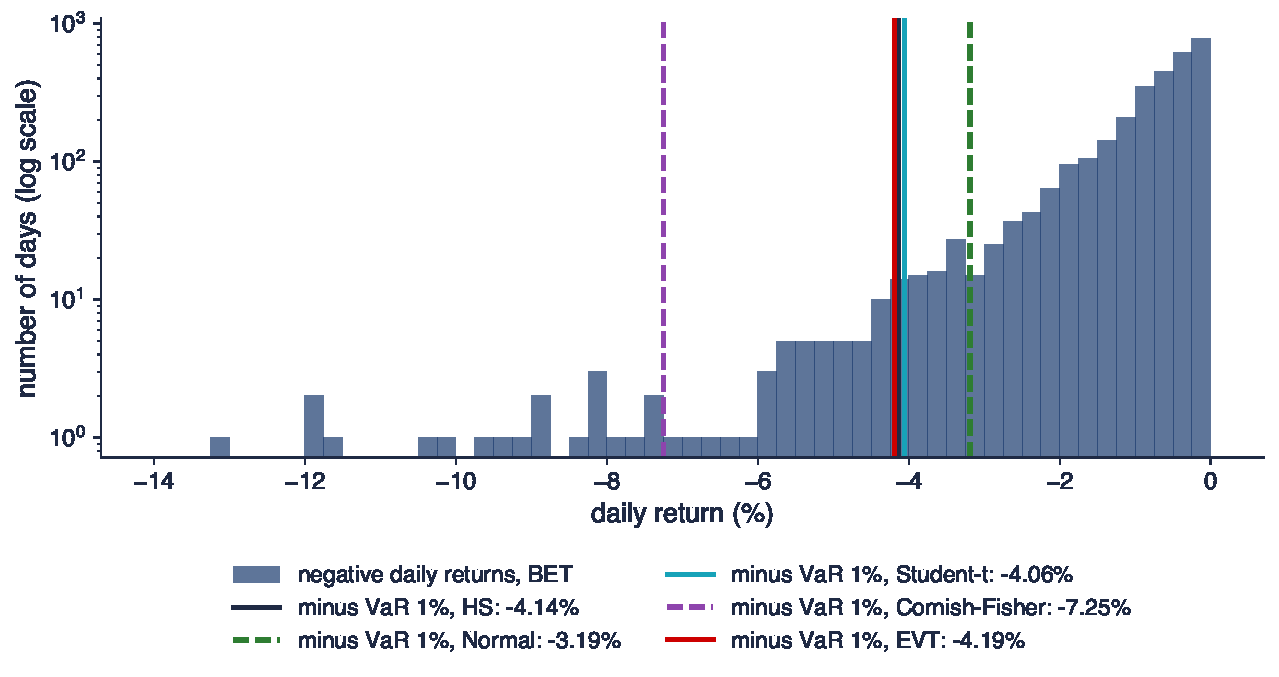
\includegraphics[width=0.96\textwidth,height=0.30\textheight,keepaspectratio]{ch10_sem_b1.pdf}
\end{center}
\vspace{-2mm}
\begin{center}
\scriptsize
\begin{tabular}{lrrrrr}
\toprule
& HS & Normal & Student-t & Cornish--Fisher & EVT \\
\midrule
VaR 1\% & $4.14$ & $3.19$ & $4.06$ & $7.25$ & $4.19$ \\
ES 2.5\% & $4.57$ & $3.21$ & $4.76$ & $7.93$ & $4.57$ \\
\bottomrule
\end{tabular}
\end{center}
\begin{itemize}
    \item $n = 6\,670$; $\hat\mu = 0.064$, $\hat\sigma = 1.40$; $S = -0.65$, $K = 11.1$; $\hat\nu = 2.43$; EVT: $u = 1.24\%$, $N_u = 667$, $\hat\xi = 0.23$
    \item The Normal VaR 1\% is 23\% below the data; Cornish--Fisher ($z_{CF} = -5.23$) is far above all others
    \item Interpretation: report the historical or the EVT value (about 4.14\% and 4.57\%), which agree; mention that the Normal understates and Cornish--Fisher is outside its range with $K > 10$
\end{itemize}\sfmquantlet{Ch_10}{SFM_ch10_seminar}
\end{frame}

\begin{frame}{B2: TLV, SNP and Bitcoin [Proposed]}
\itemsize{\footnotesize}
\begin{itemize}
\item \textbf{Question}: does the ranking of the methods found for the BET hold for two BVB stocks and for Bitcoin? Model: B1.
\item \textbf{Inputs}: TLV and SNP since 2010 (TLV without 30--31 May 2016), Bitcoin since 2014; daily log returns in \%
\item \textbf{Tasks}
\begin{enumerate}
    \item Compute VaR 1\% and ES 2.5\% of each series by the five methods of B1.
    \item Compute by how much the Normal VaR 1\% is below the historical VaR 1\%.
    \item Report $\hat\nu$, $\hat\xi$ and the excess kurtosis of each series.
    \item Interpretation: for which series does the Normal understate VaR 1\% most?
\end{enumerate}
\item \textbf{Report}: one table and two sentences
\item Notebook: section B2
\end{itemize}
\end{frame}

\ifsolutions
\begin{frame}{B2: Solution [Proposed]}
\itemsize{\footnotesize}
\begin{center}
\scriptsize
\begin{tabular}{l|rrrrr|rrr|rr}
\toprule
& \multicolumn{5}{c|}{VaR 1\%} & \multicolumn{3}{c|}{ES 2.5\%} & & \\ & HS & N & t & CF & EVT & HS & N & EVT & gap N & $K$ \\
\midrule
TLV & $5.11$ & $4.01$ & $4.63$ & $10.19$ & $4.90$ & $5.37$ & $4.03$ & $5.35$ & 22\% & ${13.5}$ \\
SNP & $4.29$ & $3.70$ & $4.26$ & $7.55$ & $4.38$ & $4.70$ & $3.72$ & $4.71$ & 14\% & ${8.9}$ \\
Bitcoin & $10.54$ & $7.99$ & $11.06$ & $18.89$ & $10.38$ & $10.84$ & $8.03$ & $10.90$ & 24\% & ${12.0}$ \\
\bottomrule
\end{tabular}
\end{center}
\begin{itemize}
    \item N: Normal, t: Student-t, CF: Cornish--Fisher; gap N: how much the Normal VaR 1\% is below HS
    \item The ranking of B1 holds: Normal too low, CF far too high, HS and EVT close; $\hat\nu$: TLV $3.44$, SNP $3.79$, Bitcoin $2.23$; $\hat\xi$: $0.26$, $0.22$, $0.12$
    \item Interpretation: Bitcoin (24\%) and TLV (22\%): the heaviest tails relative to the variance; SNP has the smallest gap
\end{itemize}\sfmquantlet{Ch_10}{SFM_ch10_seminar}
\end{frame}
\fi

\begin{frame}{B3: Backtesting the S\&P 500 Year by Year [Solved]}
\itemsize{\footnotesize}
\begin{itemize}
\item \textbf{Question}: which of two VaR 1\% models would a supervisor have penalised, year by year, since 2015?
\item \textbf{Inputs}: S\&P 500 since 2000; forecasts for every day since 2 January 2015
\item \textbf{Tasks}
\begin{enumerate}
    \item Compute the one-day VaR 1\% by historical simulation on the last 250 days.
    \item Compute the one-day GARCH(1,1)-t VaR 1\%, re-estimating the model at the start of every year on all earlier data.
    \item Count the exceptions of each model in every calendar year and give the Basel zone of each year.
    \item Run the Kupiec and Christoffersen tests on the whole period.
    \item Interpretation: which model would a supervisor have penalised in 2022?
\end{enumerate}
\item \textbf{Report}: the chart, six statistics with p-values and two sentences
\item Notebook: section B3
\end{itemize}
\end{frame}

\begin{frame}{B3: Solution [Solved]}
\itemsize{\scriptsize}
\begin{center}
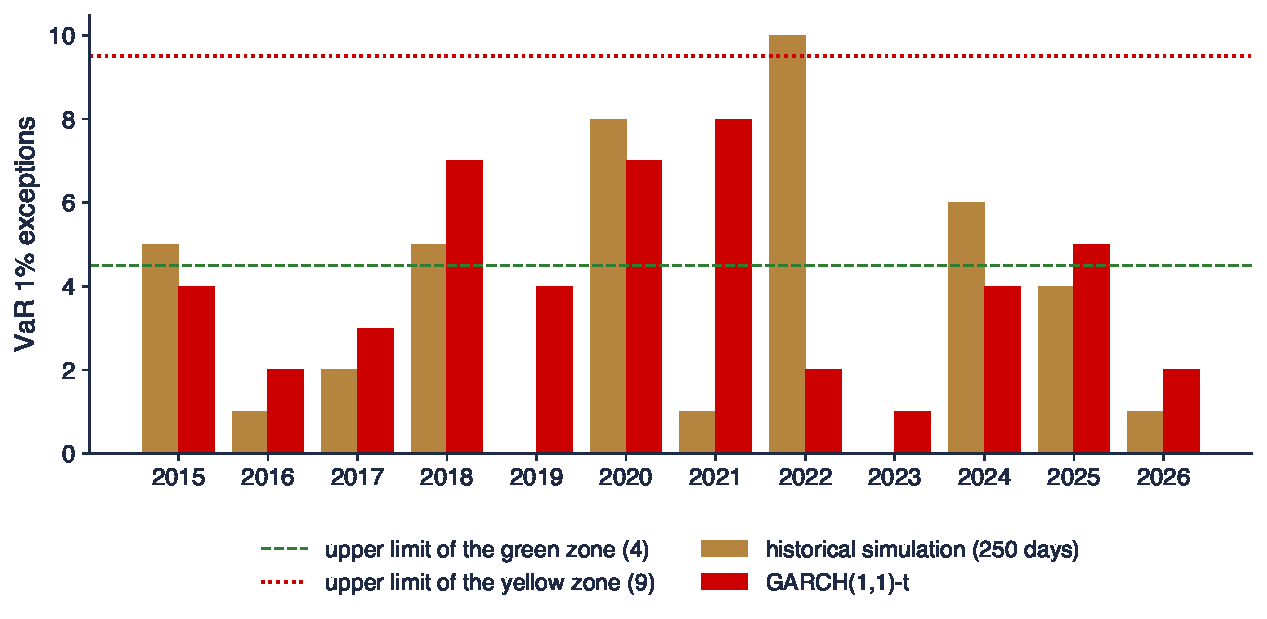
\includegraphics[width=0.96\textwidth,height=0.34\textheight,keepaspectratio]{ch10_sem_b3.pdf}
\end{center}
\vspace{-2mm}
\begin{center}
\scriptsize
\begin{tabular}{lrrrrrrr}
\toprule
& $n$ & $x$ & rate (\%) & $LR_{uc}$ (p) & $LR_{ind}$ (p) & $LR_{cc}$ (p) & red/yellow years \\
\midrule
HS 250 & 2\,944 & 43 & $1.46$ & $5.52$ (0.019) & $23.04$ ($<$\,0.001) & $28.56$ ($<$\,0.001) & 1/4 \\
GARCH-t & 2\,944 & 49 & $1.66$ & $10.94$ ($<$\,0.001) & $6.78$ (0.009) & $17.72$ ($<$\,0.001) & 0/4 \\
\bottomrule
\end{tabular}
\end{center}
\begin{itemize}
    \item Both models are exceeded too often (expected about 29.4); HS exceptions cluster strongly ($n_{11} = 7$, p ind.\ $<$\,0.001), GARCH-t less ($n_{11} = 4$)
    \item Interpretation: in 2022 HS had 10 exceptions (red zone), GARCH-t 2: the slow window was penalised when volatility rose; GARCH-t paid in calmer years (2021: 8)
\end{itemize}\sfmquantlet{Ch_10}{SFM_ch10_seminar}
\end{frame}

\begin{frame}{B4: Backtesting the BET and Bitcoin [Proposed]}
\itemsize{\footnotesize}
\begin{itemize}
\item \textbf{Question}: does the conclusion of B3 hold on the BVB and for Bitcoin? Model: B3.
\item \textbf{Inputs}: BET since 2000, forecasts since 2015; Bitcoin since 2014, forecasts since 2016
\item \textbf{Tasks}
\begin{enumerate}
    \item Compute both VaR 1\% forecasts as in B3.
    \item Count the exceptions per calendar year and give the zones.
    \item Run the Kupiec and Christoffersen tests on the whole period.
    \item Interpretation: which model would you keep for each series?
\end{enumerate}
\item \textbf{Report}: one table and two sentences
\item Notebook: section B4
\end{itemize}
\end{frame}

\ifsolutions
\begin{frame}{B4: Solution [Proposed]}
\itemsize{\footnotesize}
\begin{center}
\scriptsize
\begin{tabular}{llrrrrrrr}
\toprule
& & $n$ & $x$ & rate (\%) & p POF & p ind. & p c.c. & red/yellow years \\
\midrule
BET & HS 250 & 2\,926 & 43 & $1.47$ & 0.017 & 0.003 & $<$\,0.001 & 0/2 \\
 & GARCH-t & 2\,926 & 34 & $1.16$ & 0.391 & 0.371 & 0.464 & 0/3 \\
Bitcoin & HS 250 & 3\,914 & 40 & $1.02$ & 0.891 & 0.069 & 0.190 & 0/2 \\
 & GARCH-t & 3\,914 & 50 & $1.28$ & 0.094 & 0.672 & 0.226 & 0/5 \\
\bottomrule
\end{tabular}
\end{center}
\begin{itemize}
    \item BET: GARCH-t passes all three tests (rate 1.16\%); HS is exceeded too often and its exceptions cluster
    \item Bitcoin: HS passes (rate 1.02\%); GARCH-t is borderline (1.28\%, p POF 0.094) with 5 yellow years
    \item Interpretation: keep GARCH-t for the BET and HS (or FHS) for Bitcoin: the best method depends on the market, so every model needs its own backtest
\end{itemize}\sfmquantlet{Ch_10}{SFM_ch10_seminar}
\end{frame}
\fi

\begin{frame}{B5: A Portfolio of Two BVB Stocks [Solved]}
\itemsize{\footnotesize}
\begin{itemize}
\item \textbf{Question}: how much does diversification between Banca Transilvania and OMV Petrom reduce VaR 1\%, and does it survive a crisis?
\item \textbf{Inputs}: TLV and SNP adjusted closes since 2010, joined on common days; simple returns in \%; weights 50/50
\item \textbf{Tasks}
\begin{enumerate}
    \item Compute the variance--covariance VaR 1\% of the portfolio, the two individual VaRs and the diversification benefit.
    \item Compute the historical VaR 1\% and ES 2.5\% of the portfolio.
    \item Compute the correlation in 2017 and in February--May 2020, and the tail dependence at $q = 5\%$ and $q = 1\%$.
    \item Fit a t copula and compute the copula VaR 1\% with empirical margins.
    \item Interpretation: why does the variance--covariance VaR understate the risk of this portfolio?
\end{enumerate}
\item \textbf{Report}: eight numbers, the chart and two sentences
\item Notebook: section B5
\end{itemize}
\end{frame}

\begin{frame}{B5: Solution [Solved]}
\itemsize{\scriptsize}
\begin{center}
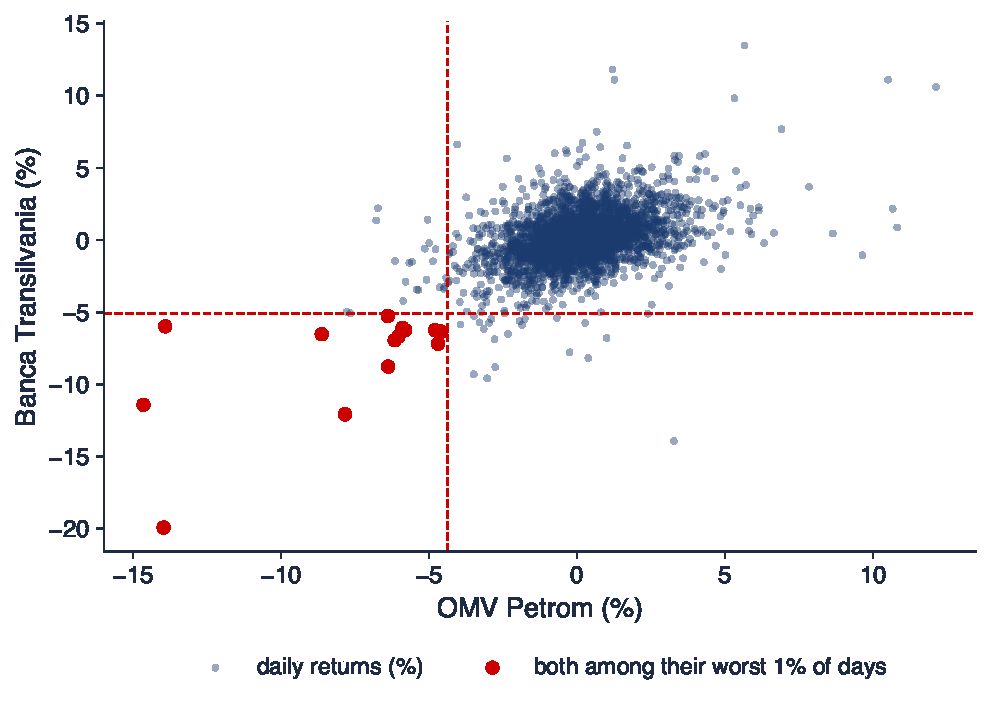
\includegraphics[width=0.96\textwidth,height=0.32\textheight,keepaspectratio]{ch10_sem_b5.pdf}
\end{center}
\vspace{-2mm}
\begin{itemize}
    \item $n = 3\,461$; $\hat\sigma$: TLV $1.84$, SNP $1.70$; $\hat\rho = 0.46$; $\sigma_p = 1.511$; VaR 1\%: TLV $4.17$, SNP $3.85$, portfolio $3.41\%$; benefit 15\%
    \item Historical: VaR 1\% $= 4.12\%$, ES 2.5\% $= 4.51\%$; t copula ($\hat\nu = 5.00$, $\lambda = 0.166$): VaR 1\% $= 3.96\%$
    \item Correlation: 2017 $0.32$, spring 2020 $0.69$; tail dependence $0.36$ ($q = 5\%$), $0.40$ ($q = 1\%$); joint worst-1\% days: 14, against 0.35 under independence
    \item Interpretation: the Normal VaR is 17\% below the historical one: both margins have heavy tails and the two stocks fall together on the worst days, when the correlation is highest
\end{itemize}\sfmquantlet{Ch_10}{SFM_ch10_seminar}
\end{frame}

\begin{frame}{B6: DAX and S\&P 500 [Proposed]}
\itemsize{\footnotesize}
\begin{itemize}
\item \textbf{Question}: is the Gaussian copula good enough for a 50/50 DAX and S\&P 500 portfolio? Model: B5.
\item \textbf{Inputs}: DAX and S\&P 500 closes since 2000, joined on common days; simple returns in \%
\item \textbf{Tasks}
\begin{enumerate}
    \item Compute the variance--covariance and the historical VaR 1\% and ES 2.5\%.
    \item Fit the Gaussian and the t copula and compare them with the LR statistic.
    \item Compute the copula VaR 1\% and ES 2.5\% with empirical margins for both copulas.
    \item Interpretation: is the Gaussian copula good enough for this pair?
\end{enumerate}
\item \textbf{Report}: one table and two sentences
\item Notebook: section B6
\end{itemize}
\end{frame}

\ifsolutions
\begin{frame}{B6: Solution [Proposed]}
\itemsize{\footnotesize}
\begin{center}
\footnotesize
\begin{tabular}{lrr}
\toprule
Method & VaR 1\% & ES 2.5\% \\
\midrule
variance--covariance & $2.72$ & $2.74$ \\
Gaussian copula & $3.22$ & $3.34$ \\
t copula & $3.35$ & $3.51$ \\
historical simulation & $3.36$ & $3.57$ \\
\bottomrule
\end{tabular}
\end{center}
\begin{itemize}
    \item $n = 6\,605$; $\hat\rho = 0.60$, $\hat\tau = 0.387$, copula $\rho = 0.571$; t copula $\hat\nu = 3.00$, LR $= 611.4$ against the Gaussian copula, $\lambda = 0.355$
    \item The t copula reproduces the historical VaR 1\% almost exactly; the Gaussian copula is lower, the variance--covariance VaR lower still
    \item Interpretation: no: two developed markets that trade at overlapping hours have strong tail dependence ($\lambda = 0.355$), which only the t copula captures
\end{itemize}\sfmquantlet{Ch_10}{SFM_ch10_seminar}
\end{frame}
\fi


%=============================================================================
\section{Part C: Open Questions and AI Critique}
%=============================================================================

\begin{frame}{C1: Is ES 2.5\% as Large as VaR 1\%? [Proposed]}
\itemsize{\footnotesize}
\begin{itemize}
\item \textbf{Question}: Basel replaced VaR 1\% by ES 2.5\% because the two are equal for Normal returns; how close are they on real data and in crises?
\item \textbf{Inputs}: S\&P 500, DAX, BET, Bitcoin, TLV, SNP, BRD; models: B1, A5
\item \textbf{Tasks}
\begin{enumerate}
    \item Compute the ratio ES 2.5\% / VaR 1\% by historical simulation on the whole sample of each series.
    \item Compute the same ratio on the 500 days that end in March 2009 and in May 2020.
    \item Compute the ratio implied by a fitted Student-t distribution.
    \item Interpretation: is ES 2.5\% a stricter rule than VaR 1\% on these markets?
\end{enumerate}
\item \textbf{Report}: a table and a plan for a project
\item Notebook: section C1
\end{itemize}
\end{frame}

\ifsolutions
\begin{frame}{C1: Reference Analysis [Proposed]}
\itemsize{\footnotesize}
\begin{center}
\scriptsize
\begin{tabular}{lrrrrr}
\toprule
& all data & 500 d. to 3/2009 & 500 d. to 5/2020 & Student-t & $\hat\nu$ \\
\midrule
S\&P 500 & $1.09$ & $0.97$ & $1.10$ & $1.14$ & $2.7$ \\
DAX & $1.01$ & $0.90$ & $1.26$ & $1.11$ & $3.1$ \\
BET & $1.10$ & $0.89$ & $1.06$ & $1.17$ & $2.4$ \\
Bitcoin & $1.03$ & -- & $1.21$ & $1.21$ & $2.2$ \\
TLV & $1.05$ & -- & $1.12$ & $1.09$ & $3.4$ \\
SNP & $1.10$ & -- & $1.09$ & $1.07$ & $3.8$ \\
BRD & $1.04$ & -- & $1.09$ & $1.05$ & $4.7$ \\
\bottomrule
\end{tabular}
\end{center}
\begin{itemize}
    \item Normal: $1.005$; the data: from $0.89$ to $1.26$; Bitcoin and the BVB stocks have no data before 2009
    \item The ratio can be below 1 (windows ending in 2009): one huge loss pushes VaR 1\% up more than the average ES 2.5\%
    \item Project design: rolling ratios for many assets, bootstrap intervals (the ratio is noisy), the link with the tail index $\xi$ (\sfmchlink{https://danpele.github.io/SFM/EN/Courses/chapter5_heavy_tails_evt.pdf}{Chapter 5}), and the capital that each rule would require
\end{itemize}\sfmquantlet{Ch_10}{SFM_ch10_seminar}
\end{frame}
\fi

\begin{frame}{C2: Audit an AI Answer [Proposed]}
\itemsize{\scriptsize}
\begin{itemize}
    \item A student asked an AI assistant to summarise the risk of the BET over the last 500 days. The answer:
    \item \aiprompt{(a) The VaR 99\% of the BET is -2.93\%.}
    \item \aiprompt{(b) ES is always at least as large as VaR, so ES 2.5\% is above 2.93\%.}
    \item \aiprompt{(c) The 10-day VaR 1\% is 10 x 2.93 = 29.3\%.}
    \item \aiprompt{(d) With 8 exceptions in 250 days the Kupiec p-value is 0.005, but the model stays in the green zone.}
    \item \aiprompt{(e) VaR is subadditive, so the VaR of a portfolio never exceeds the sum of the VaRs of its parts.}
    \item \aiprompt{(f) If the exceptions cluster, the Christoffersen test can reject even when their number is right.}
    \item Tasks
    \begin{itemize}
        \item 1. For each statement, say whether it is correct; if not, give the correct statement and, where possible, the correct number from the notebook (section C2).
        \item 2. Report: a list of six verdicts with one line of justification each.
    \end{itemize}
\end{itemize}
\end{frame}

\ifsolutions
\begin{frame}{C2: Solution [Proposed]}
\itemsize{\footnotesize}
\begin{itemize}
    \item (a) Wrong twice: the level is the tail probability (VaR 1\%), and VaR is a loss, a positive number: VaR 1\% $= 2.93\%$
    \item (b) Wrong: $\mathrm{ES}_\alpha \ge \mathrm{VaR}_\alpha$ only at the same level; here ES 2.5\% $= 2.69\%$ is below VaR 1\% (A3)
    \item (c) Wrong: the square-root-of-time rule gives $\sqrt{10} \times 2.93 = 9.25\%$, and even that holds only for i.i.d.\ Normal returns
    \item (d) Wrong: 8 exceptions are in the yellow zone (plus factor 0.75); $LR_{uc} = 7.73$ also rejects the model
    \item (e) Wrong: VaR can fail subadditivity (the two bonds of A4); ES is the coherent measure
    \item (f) Correct: this is the independence part of the conditional coverage test (A6)
\end{itemize}\sfmquantlet{Ch_10}{SFM_ch10_seminar}
\end{frame}
\fi


%=============================================================================
\section{Wrap-Up}
%=============================================================================

\begin{frame}{What You Should Take from Today}
\itemsize{\small}
\begin{itemize}
    \item VaR 1\% $= -q_{1\%}$, a positive loss; ES 2.5\% averages the worst 2.5\% of days; ES $\ge$ VaR only at the same level
    \item On real data the Normal method understates VaR; Cornish--Fisher fails for large kurtosis; HS and EVT agree at 1\%
    \item Backtesting needs two checks: the number of exceptions (Kupiec) and their independence (Christoffersen)
    \item Diversification is weakest in crises: correlation and tail dependence rise together
    \item An AI answer is a draft: check the sign and the level of VaR, the horizon rule and the Basel zone
\end{itemize}
\end{frame}

\begin{frame}{After the Seminar}
\itemsize{\small}
\begin{itemize}
    \item Lecture 10 develops each topic of today: definitions and coherence, estimation methods, conditional VaR, portfolios and copulas, backtesting
    \item Try the [Proposed] tasks in the notebook; the solutions are discussed in class
    \item C1 can grow into a team project: rolling ratios, bootstrap intervals, the capital under each rule
    \item Reading: \refFHH, Ch.~16; exercises in \refBHL, Ch.~16; \refQRM, Ch.~2
\end{itemize}
\end{frame}


%=============================================================================
\section{References}
%=============================================================================

\begin{frame}{References}
\itemsize{\tiny}
\begin{itemize}
    \item Acerbi, C., Tasche, D. (2002). \href{https://doi.org/10.1016/S0378-4266(02)00283-2}{On the coherence of expected shortfall}. \textit{Journal of Banking \& Finance}, 26(7), 1487--1503.
    \item Artzner, P., Delbaen, F., Eber, J.-M., Heath, D. (1999). \href{https://doi.org/10.1111/1467-9965.00068}{Coherent measures of risk}. \textit{Mathematical Finance}, 9(3), 203--228.
    \item Basel Committee on Banking Supervision (1996b). \href{https://www.bis.org/publ/bcbs22.htm}{Supervisory framework for the use of ``backtesting'' in conjunction with the internal models approach to market risk capital requirements}. Bank for International Settlements.
    \item Borak, S., Härdle, W.K., López-Cabrera, B. (2013). \href{https://doi.org/10.1007/978-3-642-33929-5}{\textit{Statistics of Financial Markets: Exercises and Solutions}}, 2nd ed. Springer.
    \item Christoffersen, P.F. (1998). \href{https://doi.org/10.2307/2527341}{Evaluating interval forecasts}. \textit{International Economic Review}, 39(4), 841--862.
    \item Cornish, E.A., Fisher, R.A. (1938). \href{https://doi.org/10.2307/1400905}{Moments and cumulants in the specification of distributions}. \textit{Revue de l'Institut International de Statistique}, 5(4), 307--320.
    \item Demarta, S., McNeil, A.J. (2005). \href{https://doi.org/10.1111/j.1751-5823.2005.tb00254.x}{The t copula and related copulas}. \textit{International Statistical Review}, 73(1), 111--129.
    \item Franke, J., Härdle, W.K., Hafner, C.M. (2019). \href{https://doi.org/10.1007/978-3-030-13751-9}{\textit{Statistics of Financial Markets: An Introduction}}, 5th ed. Springer.
    \item Kupiec, P.H. (1995). \href{https://doi.org/10.3905/jod.1995.407942}{Techniques for verifying the accuracy of risk measurement models}. \textit{Journal of Derivatives}, 3(2), 73--84.
    \item McNeil, A.J., Frey, R. (2000). \href{https://doi.org/10.1016/S0927-5398(00)00012-8}{Estimation of tail-related risk measures for heteroscedastic financial time series: an extreme value approach}. \textit{Journal of Empirical Finance}, 7(3--4), 271--300.
    \item McNeil, A.J., Frey, R., Embrechts, P. (2015). \href{https://press.princeton.edu/books/hardcover/9780691166278/quantitative-risk-management}{\textit{Quantitative Risk Management: Concepts, Techniques and Tools}}, revised ed. Princeton University Press.
\end{itemize}
\end{frame}

\end{document}
